\documentclass{article}[a4paper, oneside, 11pt]
\synctex=1
\usepackage[T1]{fontenc}
\usepackage[utf8]{inputenc}
\usepackage{calc}
\usepackage{amsmath, amssymb, amsthm, thmtools, amsfonts}
\usepackage{mathtools}
\usepackage[nochapters,pdfspacing]{classicthesis}
%\usepackage{hyperref}% clashes with classicthesis
\usepackage{cleveref}
\usepackage[siunitx]{circuitikz}
\usepackage{booktabs}
\usepackage{graphicx}
\usepackage{caption}
\usepackage{subcaption}
\usepackage{geometry}
\usepackage{float}
\usepackage{mdframed}
\usepackage{xcolor}
\usepackage{siunitx}
\usepackage[italian]{babel}
\usepackage{pgfplots}
\usepackage{titling}
\usepackage{listings}
%\usepackage{lmodern}
\usepackage{url}
\usepgfplotslibrary{external}
\tikzexternalize

\pgfplotsset{compat=1.15}
\lstset{
language=Python,
basicstyle=\ttfamily,
columns=fullflexible,
keepspaces=true,
}
\mdfsetup{linewidth=0.6pt}
\graphicspath{{./figs/}}
\makeatletter
\def\input@path{{./figs/}}
%or: \def\input@path{{/path/to/folder/}{/path/to/other/folder/}}
\makeatother

% Default fixed font does not support bold face
\DeclareFixedFont{\ttb}{T1}{txtt}{bx}{n}{12} % for bold
\DeclareFixedFont{\ttm}{T1}{txtt}{m}{n}{12}  % for normal

% Custom colors
\usepackage{color}
\definecolor{deepblue}{rgb}{0,0,0.5}
\definecolor{deepred}{rgb}{0.6,0,0}
\definecolor{deepgreen}{rgb}{0,0.5,0}

% Commands 
\newcommand{\executeiffilenewer}[3]{%
	\ifnum\pdfstrcmp{\pdffilemoddate{#1}}%
		{\pdffilemoddate{#2}}>0%
	{\immediate\write18{#3}}\fi%
}
% input .svg --> .pdf_tex graphs
\newcommand{\includesvg}[1]{%
	\executeiffilenewer{#1.svg}{#1.pdf}%
	{inkscape -z -D --file=#1.svg %
	--export-pdf=#1.pdf --export-latex}%
	\input{#1.pdf_tex}%
}

\newcommand{\eps}{\varepsilon}
\renewcommand{\phi}{\varphi}
\newcommand{\loc}{\mathit{loc}}
\newcommand{\weakto}{\rightharpoonup}
\newcommand{\implied}{\Longleftarrow}
\let\subsetstrict\subset
\renewcommand{\subset}{\subseteq}
\renewcommand{\supset}{\supseteq}

% calligraphic letters
\newcommand{\A}{\mathcal A}
\newcommand{\B}{\mathcal B}
\newcommand{\C}{\mathcal C}
\newcommand{\D}{\mathcal D}
\newcommand{\E}{\mathcal E}
\newcommand{\F}{\mathcal F}
\newcommand{\FL}{\mathcal F\!\mathcal L}
\renewcommand{\H}{\mathcal H}
\newcommand{\K}{\mathcal K}
\renewcommand{\L}{\mathcal L}
\newcommand{\M}{\mathcal M}
\renewcommand{\P}{\mathcal P}
\renewcommand{\S}{\mathcal S}
\newcommand{\U}{\mathcal U} %% intorni

% blackboard letters
\newcommand{\CC}{\mathbb C}
\newcommand{\HH}{\mathbb H}
\newcommand{\KK}{\mathbb K}
\newcommand{\NN}{\mathbb N}
\newcommand{\QQ}{\mathbb Q}
\newcommand{\RR}{\mathbb R}
\newcommand{\TT}{\mathbb T}
\newcommand{\ZZ}{\mathbb Z}

\newcommand{\Abs}[1]{{\left\Vert #1\right\Vert}}
\newcommand{\enclose}[1]{{\left( #1 \right)}}
\newcommand{\Enclose}[1]{{\left[ #1 \right]}}
\newcommand{\floor}[1]{\left\lfloor #1 \right\rfloor}
\newcommand{\ceil}[1]{\left\lceil #1 \right\rceil}

\newcommand{\To}{\rightrightarrows}
\renewcommand{\vec}[1]{\boldsymbol #1}
\newcommand{\defeq}{:=}
\DeclareMathOperator{\divergence}{div}
\renewcommand{\div}{\divergence}
\DeclareMathOperator{\Imaginarypart}{Im}
\renewcommand{\Im}{\Imaginarypart}
\DeclareMathOperator{\Realpart}{Re}
\renewcommand{\Re}{\Realpart}
%\DeclareMathOperator{\arg}{arg}
\DeclareMathOperator{\tg}{tg}
\DeclareMathOperator{\arctg}{arctg}
\DeclareMathOperator{\settsinh}{settsinh}
\DeclareMathOperator{\settcosh}{settcosh}
\DeclareMathOperator{\tr}{tr}
\DeclareMathOperator{\im}{im}
\DeclareMathOperator{\sgn}{sgn}
\DeclareMathOperator{\diag}{diag}

\declaretheoremstyle[
spaceabove=6pt, spacebelow=6pt,
headfont=\normalfont\bfseries\itshape,
notefont=\mdseries, notebraces={(}{)},
bodyfont=\normalfont,
postheadspace=1em,
qed=,
%shaded={rulecolor=pink!30,rulewidth=1pt,bgcolor=pink!10}
]{exercise_style}

\declaretheoremstyle[
spaceabove=6pt, spacebelow=6pt,
postheadspace=1em,
qed=,
%shaded={rulecolor=blue!20,rulewidth=1pt,bgcolor=blue!5}
]{theorem_style}

\declaretheoremstyle[
spaceabove=6pt, spacebelow=6pt,
postheadspace=1em,
qed=,
%shaded={rulecolor=yellow!50,rulewidth=1pt,bgcolor=yellow!5}
]{axiom_style}

\declaretheorem[name=Teorema]{theorem}
\declaretheorem[name=Lemma,sibling=theorem]{lemma}
\declaretheorem[name=Proposizione,sibling=theorem]{proposition}
\declaretheorem[name=Corollario,sibling=theorem]{corollary}
\declaretheorem[name=Paradosso,sibling=theorem]{paradox}
\declaretheorem[style=axiom_style,name=Assioma,sibling=theorem]{axiom}
\declaretheorem[name=Definizione,sibling=theorem]{definition}
\declaretheorem[style=exercise_style,name=Esempio,sibling=theorem]{example}
\declaretheorem[style=exercise_style,name=Esercizio,sibling=theorem]{exercise}
\declaretheorem[style=exercise_style,name=Osservazione,sibling=theorem]{remark}

% Logarithm with arbitrary base.
% -> log_10
\newcommand{\llog}[1][10]{\log_{#1}}

% Absolute value.
% -> |x|
\newcommand{\abs}[1]{\left| #1 \right|}

% Powers.
% -> x^a
\newcommand{\power}[2][2]{\left( #2 \right)^{#1}}

% Square.
% -> x^2
\newcommand{\sq}[1]{\power[2]{#1}}

% Expansion of the binomial coefficient.
% -> n1!/(n2!(n1 - n2)!)
\newcommand{\binomexpr}[2]{\frac{#1!}{#2!(#1 - #2)!}}

% Expression evaluation at a given point with square brackets.
% -> [x]_{a}
\newcommand{\at}[2]{\left[ #1\right]_{\makebox[-1pt][l]{${\scriptstyle#2}$}}}

% Expression evaluation in an interval.
% -> [x] _{a}^{b}
\newcommand{\eval}[3]{\left.#1%
  \right|_{\makebox[-1pt][l]{${\scriptstyle#2}$}}^{\makebox[-1pt][l]{${\scriptstyle#3}$}}}

% Upright d in math mode (for differentials).
% -> d
\newcommand{\ud}{\mathrm{d}}

% Differential.
% -> dx
\newcommand{\diff}[1][x]{\,\ud{#1}}

% Base command for defining derivatives.
% -> df/dx or d^kf/dx^k
\newcommand{\basederivative}[4][]{%
  \displaystyle%
  \ifx\\#1\\\frac{#4#2}{#4#3}%
  \else%
  \frac{#4^#1#2}{#4#3^#1}%
  \fi%
}

% Total derivative.
% -> df/dx(x) or d^kf/dx^k(x)
\newcommand{\td}[4][]{%
  \basederivative[#1]{#2}{#3}{\ud}%
  \ifx\\#4\\%
  \else%
  \mkern-4mu\left(#4\right)%
  \fi%
}

% Partial derivative.
% -> df/dx(x) or d^kf/dx^k(x)
\newcommand{\pd}[4][]{%
  \basederivative[#1]{#2}{#3}{\partial}%
  \ifx\\#4\\%
  \else%
  \mkern-4mu\left(#4\right)%
  \fi%
}

\newcommand{\intinf}{\int_{-\infty}^{\infty}\!\!\!}

\newcommand{\cinterval}[2]{\left[\, #1,~#2 \,\right]}

\newcommand{\linterval}[2]{\left[\, #1,~#2 \,\right)}

\newcommand{\rinterval}[2]{\left(\, #1,~#2 \,\right]}

\newcommand{\ointerval}[2]{\left(\, #1,~#2 \,\right)}

\newcommand{\prob}[1]{\displaystyle P\left(#1\right)}

\newcommand{\pvalue}{\emph{$p$-value}}

\newcommand{\cond}{\,|\,}

\newcommand{\expect}[1]{\displaystyle E\left[#1\right]}

\newcommand{\mom}[2][]{\displaystyle {\cal M}_{#2}\ifx\\#1\\\else(#1)\fi}

\newcommand{\momalg}[1]{\displaystyle \lambda_{#1}}

\newcommand{\momcen}[1]{\displaystyle \mu_{#1}}

\newcommand{\skewness}{\displaystyle \gamma_1}

\newcommand{\kurtosis}{\displaystyle \gamma_2}

\newcommand{\charf}[1][x]{\phi_{#1}}

\newcommand{\momgenf}[1][x]{M_{#1}}

\newcommand{\fwhm}{{\scriptstyle \textsc{FWHM}}}

\newcommand{\hwhm}{{\scriptstyle \textsc{HWHM}}}

\newcommand{\median}{\mu_{\nicefrac{1}{2}}}

\newcommand{\var}[1]{\ensuremath{\text{Var}\left(#1\right)}}

\newcommand{\cov}[2]{\ensuremath{\text{Cov}\left(#1, #2\right)}}

\newcommand{\corr}[2]{\ensuremath{\text{Corr}\left(#1, #2\right)}}

\newcommand{\like}{\mathcal L}

\newcommand{\likelihood}[2][]{\like\ifx\\#2\\\else(#2\ifx\\#1\\\else;#1\fi)\fi}

\newcommand{\chisq}{\ensuremath{\chi^2}}

\newcommand{\chisquare}[2][]{\chisq\ifx\\#2\\\else(#2\ifx\\#1\\\else;#1\fi)\fi}

\newcommand{\loglikelihood}[2][]{\log\likelihood[#1]{#2}}

\newcommand{\pdf}[3][]{#2(#3\ifx\\#1\\\else;#1\fi)}

\newcommand{\binomialpdf}[2][]{\pdf[#1]{\mathcal B}{#2}}

\newcommand{\multinomialpdf}[2][]{\pdf[#1]{\mathcal M}{#2}}

\newcommand{\poissonpdf}[2][]{\pdf[#1]{\mathcal P}{#2}}

\newcommand{\uniformpdf}[2][]{\pdf[#1]{u}{#2}}

\newcommand{\exponentialpdf}[2][]{\pdf[#1]{\varepsilon}{#2}}

\newcommand{\gausspdf}[2][]{\pdf[#1]{N}{#2}}

\newcommand{\chisquarepdf}[2][]{\pdf[#1]{\wp}{#2}}

\newcommand{\cauchypdf}[2][]{\pdf[#1]{c}{#2}}

\newcommand{\erf}[1]{\ensuremath{\text{erf}\left(#1\right)}}

\newcommand{\dccases}[4][]{#2 \ifx\\#2\\\else=\fi %
  \begin{cases}
    \displaystyle #3 & \text{per variabili discrete}\\
    \displaystyle #4 & \text{per variabili continue}#1
  \end{cases}
}
\newcommand\Scaleforall[1]{\vcenter{\hbox{\scalefont{#1}$\forall$}}}

\DeclareMathOperator*\forevery{%
  \vphantom\sum
  \mathchoice{\Scaleforall{2}}{\Scaleforall{1.4}}{\Scaleforall{1}}{\Scaleforall{0.75}}}

\geometry{a4paper, left=25mm, right=25mm, top=25mm, bottom=25mm}
\title{Esercizio facoltativo* sulla FFT}
\author{M.~Alighieri(\thanks{Dipartimento di Fisica E.~Fermi,
		Universit\`a~di~Pisa - Pisa, Italy} )~\and
		M.~Romagnoli(\protect\footnotemark[1] )~\and 
		B.~Tomelleri(\protect\footnotemark[1] )}%

\begin{document}
\maketitle

%================================================================
%                         Introduzione
%================================================================
\section{Introduzione}
Si è rivisitato nel dominio delle frequenze lo studio di sistemi elettronici
e meccanici, finora analizzati solamente nel dominio del tempo, attraverso l'uso
di due strumenti fondamentali: la trasformata di Fourier Discreta (DFT) e la
detezione sincrona o Lock In Detection/Amplification (LIA).

%================================================================
%                         Cenni teorici
%================================================================
\section{Cenni Teorici}
La Trasformata di Fourier Discreta (o DFT) estende la trasformata di Fourier
tradizionale a sistemi con variabile dinamica discreta. In particolare
approfitteremo della velocità dell'algoritmo Cooley-Tukey \cite{FFT} o FFT
per calcolare un ciclo della DFT nella nostra analisi.

L'utilità della detezione sincrona risiede nella capacità di isolare
componenti ad una fissata frequenza e fase di un segnale da -idealmente-
tutte le fonti di rumore asincrone e fuori fase rispetto alla modulazione
di riferimento, in ambienti dove $\text{SNR} \ll 1$).
Poiché l'operazione di media temporale è svolta alla $f_{\text{ref}}$ sia
le fluttuazioni termiche ad alta frequenza o di \emph{jitter}
$\propto 1/\sqrt{T_{\text{mis}}}$ che quelle di \emph{flicker}
$\propto 1/f^\gamma$ sono mitigate dal metodo di lock-in detection.
Dal punto di vista dell'implementazione digitale un secondo pregio del LIA
risulta meno evidente (vista la possibilità di costruire filtri BPF numerici
con banda regolabile di qualità arbitraria) però, nel caso reale, costruire
filtri mobili di alta qualità $Q_f \gg 10$ è tutto fuorché banale: dunque la
possibilità di -traslare- in frequenza le componenti di un segnale rispetto
alla banda di un buon filtro "fisso" costituisce un enorme vantaggio.

\subsection{Circuito RC}
Ricordando la scomposizione di un segnale periodico in serie di Fourier,
\begin{equation}
g(t) = \frac{g_0}{2} + \sum_{k=1}^{n} b_k \cos{(\omega_kt)} + 
\sum_{k=1}^{n} c_k\sin{\left(\omega_k t\right)}
\end{equation}
possiamo estendere la descrizione dell'effetto del circuito su perturbazioni
sinusoidali a segnali periodici qualsiasi con la funzione di trasferimento:
\begin{equation}
	T(\omega_k) = \frac{1}{1 + 1/j\omega_k RC} = 
	\frac{1}{1 + j\frac{\omega_k}{\omega_T}} = \frac{1}{1 + j\frac{f_k}{f_T}}
\end{equation}
\begin{align*}\label{eq:fin}
\begin{cases}
	\mathrm{Attenuazione} \; A(\omega_k) &=
	\frac{1}{\sqrt{1 + \left(\omega_k/\omega_T \right)^2}} \\
	\mathrm{Sfasamento} \; \Delta \phi(\omega_k) &=
	\arctan{\left(- \omega_k /\omega_T \right)}
\end{cases}
\end{align*}
dove il tempo caratteristico di scarica del condensatore $\tau = RC$ definisce
la frequenza $\omega_T = 2\pi f_T = 1/RC = \frac{1}{\tau}$ 
caratteristica o di taglio del filtro.
\medskip

\subsection{Circuiti forzati e smorzati RLC}
In un circuito costituito da almeno una resistenza, un induttore ed un
condensatore (nel nostro caso collegati in serie) è possibile individuare una
frequenza caratteristica $f_0 = \frac{\omega_0}{2\pi}$, detta propria o di
risonanza, per cui il sistema è percorso da una corrente elettrica oscillante
nel tempo.
Infatti, quando il sistema è perturbato da una tensione alla frequenza
$f_0 := \frac{1}{2\pi \sqrt{LC}}$ 
le impedenze del condensatore e dell'induttore si annullano a vicenda, dunque
l'impedenza del circuito si trova al proprio valor minimo, cioè la sola
componente resistiva $R$ rimasta. Possiamo quindi descrivere il trasporto di
carica nel circuito con l'equazione di un oscillatore smorzato:
\begin{equation}\label{eq: RLC}
	\frac{\partial^2 Q}{\partial t^2} + \frac{R}{L}\frac{\partial Q}{\partial t}
	+ \omega_0^2 Q = 0   
\end{equation}
La cui soluzione, in termini della frequenza di oscillazione smorzata o
pseudo-frequenza angolare $\omega$, dello pseudo periodo $T$ e del tempo
caratteristico di smorzamento $\tau$:
\begin{align*}
	\omega &= \sqrt{\omega_0^2 - \frac{1}{\tau^2}} =
	\sqrt{\frac{1}{LC} - \frac{1}{\tau^2}} \\
	T &= \frac{2\pi}{\omega} \\
	\tau &= \frac{2L}{R}
\end{align*}
si può scrivere come:
\begin{align}\label{aln: Q(t)}
	Q(t) &= A e^{-t/\tau} \cos{(\omega t + \phi)} \\
	A &= \sqrt{c_1 c_2} \\
	\tan{\phi} &= j\frac{c_1 + c_2}{c_1 - c_2}
\end{align}
dove i coefficienti $c_1$ e $c_2$ dipendono dalle condizioni iniziali del
sistema. Secondo il nostro modello, la d.d.p. sulle armature del condensatore
è determinata dalla relazione costitutiva di $C$ e le condizioni iniziali
sono fissate dalla carica presente sulle armature $Q_0$ e dall'intensità
di corrente $I_0$ che circola nel circuito all'inizio dell'oscillazione:
\begin{align}\label{aln: Vc(t)}
	V_C(t) &= \frac{Q(t)}{C} = \frac{A}{C}e^{-\frac{t}{\tau}}\cos(\omega t + \phi)\\
	Q(t = 0) &= A\cos{\phi} := Q_0 \implies A = Q_0 \sqrt{1 + \tan^2{\phi}} \\
	I(t) &= \frac{\partial Q}{\partial t} = A e^{-t/\tau} \left[
	\frac{\cos{(\omega t + \phi)}}{\tau} + \omega\sin{(\omega t + \phi)} \right] \\
	I(t = 0) &= A \left[ \frac{\cos{\phi}}{\tau} + \omega\sin{\phi} \right] 
	\implies \phi = \arctan{\left( \frac{1}{\omega}\left[
	\frac{I_0}{Q_0} - \frac{1}{\tau}\right] \right) }
\end{align}

\subsection{Quality Factor}
Per descrivere la dissipazione media di energia da parte di sistemi oscillanti
nel tempo si è introdotta la quantità adimensionale \emph{Quality factor}:
\begin{equation}\label{eq: Qf}
	Q_f := 2\pi \frac{E_{\text{stored}}}{E_{\text{lost/cycle}}}
\end{equation}

Per un circuito RLC il trasferimento reciproco di energia elettrostatica e
magnetostatica, immagazzinate nel condensatore e nell'induttore rispettivamente,
è massimo sotto l'effetto di una forzante alla stessa $f_0$ di risonanza.
Possiamo esprimere l'energia interna all'induttore come $U_M = \frac{1}{2}LI^2$
e quella accumulata dal condensatore come $U_E = \frac{1}{2C}Q^2$.
Assumendo che all'inizio dell'oscillazione $t = 0 := t_0$ tutta l'energia del
circuito sia contenuta all'interno dell'induttore, possiamo identificare
$E_{\rm stored}$ con $U_M(t_0) := U_{M_0}$ e caratterizzare l'energia dissipata
in ogni periodo con la relazione di Joule per gli effetti termico-dissipativi:
\begin{align}
	E_{\text{stored}} =& U_{M_0} = \frac{1}{2} LI_0^2 \\
	E_{\text{lost/cycle}} =& \langle P_{\rm Joule} \rangle_t \cdot T = 
	\frac{1}{2} RI_0^2 \cdot T
\end{align}
Supponendo che il circuito sia perturbato da un segnale sinusoidale
monocromatico, il metodo simbolico ci permette di legare la larghezza di riga
della risposta in frequenza del circuito al tempo caratteristico di
smorzamento, dunque al fattore di qualità dell'oscillazione.
Nell'approssimazione di oscillazione sottosmorzata $\omega_0 \gg \frac{1}{\tau}
\implies \omega = \sqrt{\omega_0^2 - \frac{1}{\tau^2}} \approx \omega_0$
possiamo approssimare la larghezza a metà altezza della curva di risonanza con 
\begin{equation}\label{eq: FWHM}
	\Delta \omega_{\text{FWHM}}	\approx \sqrt{3} RC \omega_0^2 = 
	\sqrt{3} \frac{R}{L} = \frac{2 \sqrt{3}}{\tau} 
\end{equation}
Per cui ci si aspetta che la larghezza della campana di risonanza sia
proporzionale alla severità dello smorzamento/perdita di energia
dell'oscillazione.
In altre parole, per un circuito RLC il fattore di qualità atteso è:
\begin{equation}\label{eq: QfFWHM}
	Q_f \approx 2\pi \frac{\frac{1}{2}L I_0^2}{\frac{1}{2}R I_0^2 \cdot T_0}
	= \omega_0 \frac{L}{R} = \omega_0 \frac{\tau}{2} 
	= \sqrt{3} \frac{\omega_0}{\Delta \omega_{\text{FWHM}}} 
\end{equation}

\subsection{Oscillatore a reazione con BJT}
Il secondo tipo di sistema oscillante studiato è un circuito dotato di
un amplificatore invertente, un transistor a giunzione bipolare (BJT) montato
ad emettitore comune (emitter-follower) ed un anello di feedback.
Secondo il criterio di stabilità di Barkhausen, affinché un circuito
elettrico lineare possa sostenere la propria auto-oscillazione è necessaria
la presenza di un feedback positivo, i.e. lo sfasamento totale dovuto
all'anello di feedback dev'essere un multiplo di $2\pi$. Nel nostro caso la
condizione è soddisfatta interponendo una rete di sfasamento, costituita da
3 filtri RC passa-alto passivi, che inverte nuovamente segno
$\Delta \phi = \pi$
al segnale in uscita dall'amplificatore. Vale la pena ricordare un
modo equivalente per ottenere un sistema auto-oscillante, in cui lo stesso
sfasamento (seppur opposto in segno) è dato dalla serie di un induttore ed
un condensatore, quello che va sotto il nome di oscillatore di Colpitts.

\subsection{Detezione sincrona}
Supponiamo di voler misurare un segnale coerente, i.e. con fase costante
nel tempo $V(t)$, che per semplicità assumiamo sinusoidale -monocromatico- a
frequenza $f$, e di generare con oscillatori locali due segnali
\emph{di riferimento} $V_{\text{ri}} (t)$ e $V_{\text{rq}} (t)$ anch'essi
coerenti e sinusoidali ad una frequenza nota $f_{\text{ref}}$, ma sfasati tra
loro di $\Delta \theta = \frac{\pi}{2}$.
Moltiplicando il segnale di riferimento
$V_{\text{ri}} (t)$ per quello d'interesse $V(t)$ con un miscelatore (PSD)
si ottiene un segnale proporzionale al prodotto delle loro ampiezze e con
due componenti in frequenza, uno alla somma $f + f_{\text{ref}}$ ed uno
alla differenza $f - f_{\text{ref}}$.
\begin{align*}
	V(t) :=& V_{\text{sig}}\sin{(\omega t + \phi)} \\
	V_{\text{ri}}(t) :=& V_{\text{ref}}\sin{(\omega_{\text{ref}}t + \phi_{\text{ref}})} \\
	V_{\text{rq}}(t) :=& V_{\text{ref}}\cos{(\omega_{\text{ref}}t + \phi_{\text{ref}})} \\
	V_{\text{PSD}}(t) :=& V(t) \cdot V_{\text{ri}}(t) =
	V_{\text{sig}}\sin{(\omega t + \phi)} 
	V_{\text{ref}}\sin{(\omega_{\text{ref}}t + \phi_{\text{ref}})} = \\
	=& \frac{1}{2} V_{\text{sig}} V_{\text{ref}} \left(\cos{([\omega - 
		\omega_{\text{ref}}] + \phi - \phi_{\text{ref}}}) + 
	\cos{([\omega + \omega_{\text{ref}}] + \phi + \phi_{\text{ref}})} \right) \\
\end{align*}
Nel caso in cui anche la frequenza $f$ del segnale di nostro interesse sia
nota possiamo imporre $f_{\text{ref}} = f$, in questa configurazione "omodina"
il segnale in uscita dal detector non ha più media nulla, ma ha una componente
DC a frequenza $0 \; \si{\hertz}$ proporzionale all'ampiezza di $V(t)$.
Con un filtro passa basso possiamo allora "tagliare" il contributo dovuto
alla componente restante a $2f$, ovvero mediando sul tempo per 
$t \gg T = 1/f$, abbiamo una misura di $V_{\text{sig}}$ dipendente dallo
sfasamento $\Delta \phi = \phi - \phi_{\text{ref}}$: 
\begin{align}
	V_{\text{out}} := \langle V_{\text{PSD}} \rangle_t 
	= \frac{1}{2} V_{\text{sig}} V_{\text{ref}}\cos{(\phi - \phi_{\text{ref}})}
	\implies V_{\text{sig}}\cos{\Delta \phi} =
	2 \frac{V_{\text{out}}}{V_{\text{ref}}}
\end{align}
Per eliminare la dipendenza da $\Delta \phi$ dalla misura possiamo
ripetere lo stesso procedimento, però usando il segnale di riferimento
in quadratura $V_{\text{rq}}(t)$
\begin{align}
	V_{\text{outq}} := \langle V(t) \cdot V_{\text{rq}} (t) \rangle_t =
	\frac{1}{2} V_{\text{sig}} V_{\text{ref}}\sin{\Delta \phi}
\end{align}
Un cambio di coordinate da cartesiane a polari ci permette di esprimere in
maniera elegante il modulo e la fase del segnale da misurare $V(t)$.
\begin{align}
	X := 2 \frac{V_{\text{out}}}{V_{\text{ref}}}\cos{\Delta \phi} =
	V_{\text{sig}}\cos{\Delta \phi}; \quad
	&Y := 2 \frac{V_{\text{out}}}{V_{\text{ref}}}\sin{\Delta \phi} =
	V_{\text{sig}}\sin{\Delta \phi} \\
	V_{\text{sig}} =& \sqrt{X^2 + Y^2}\\
	\phi =& \arctan{\frac{Y}{X}}
\end{align}

%================================================================
%                Metodo e apparato sperimentale
%================================================================
\section{Metodo e apparato sperimentale}
Non si è monitorata la temperatura dei componenti dei circuiti studiati,
tutti i collegamenti tra i componenti sono stati realizzati con cavi
terminanti in connettori a banana. L'uso di \verb+Arduino+\cite{arduino}
come sistema di acquisizione dati non permette di apprezzare le perturbazioni
dovute alla temperatura o ai collegamenti dei componenti nelle nostre
condizioni di lavoro.

%================================
%           Apparato
%================================
\subsection{Apparato}
L'apparato sperimentale consiste di diversi circuiti elettrici,
realizzati con componenti pre-assemblati in laboratorio ed un generatore di
funzioni (GFG-8200A).
Per monitorare la risposta dei circuiti si utilizzano i canali di un oscilloscopio
analogico ($50$ MHz) e uno digitale ($300$ MHz), mentre per l'acquisizione dei
segnali di d.d.p. compresi tra $0$ e $5$ V si fa uso del convertitore ADC
del MCU \verb+Arduino UNO+.

\subsubsection{Circuito RC}
Si è costruito un circuito integratore RC o filtro passa-basso (LPF),
prendendo il valore nominale come riferimento per la capacità e misurando
con un multimetro digitale la resistenza in serie, le caratteristiche del
circuito risultano:
\begin{align*}
R &= 6.72 \pm 0.05 \; \si{\kilo\ohm}\\
C &= 2.2 \pm 10\% \; \si{\micro\F}\\
f_{\rm T} &= \frac{1}{2 \pi R C} = 11 \pm 1 \; \si{\hertz}
\end{align*}
Lo stesso circuito è utilizzato per i campionamenti delle forme d'onda in
uscita dal generatore di funzioni con il primo canale dell'oscilloscopio
digitale (CH1).
\begin{figure}[!htb]
	\centering
	\begin{circuitikz}[american,voltage dir=EF]
\draw (0,0)
	to[sqV, v=$V_{\rm in}$] (0,1.5) % The current source
	to [R = $r_{\rm G}$] (0,3)
	to[R = $R$, *-*] (3,3)
	to[C= $C$, -*] (3,0)
	to[short] (0,0);
\draw (0,3)
	to[short, f>^=$\text{CH1}_{\rm osc} \;V_{\rm G}$] (0,4.5)
	node[oscopeshape] {};
\draw (3,0)
	node[eground]{};
\draw (3,3)
to[short, f>_=$\text{CH2}_{\rm osc} \; V_{\text{int}}$] (3,4.5)
	node[oscopeshape] {};
\draw[gray, dashed] (-0.7, 0)--(-0.7, 3)--(0.6, 3)--(0.6, 0)--cycle;
\end{circuitikz}
	\caption{Schema circuitale dell'integratore RC realizzato in laboratorio.
	\label{fig: RC}}
\end{figure}

\subsubsection{Circuiti RLC}
Nel nostro caso l'induttore è costituito da due avvolgimenti concentrici
e coassiali, ciascuno dotato di 1500 spire, che montati in serie hanno un
fattore di auto-induzione $L \sim 0.5 \; \si{\henry}$ e i condensatori hanno
capacità dai valori nominali: $C = \left\{0.1,\; 0.22,\; 0.47\right\} \pm
10\% \; \si{\micro\farad}$. La componente resistiva $R$ del circuito è data
dalle resistenze interne del generatore di tensione ($r_G = 50 \; \si{\ohm}$
nominali) e dell'induttore, che indichiamo con: $r \approx 40 \;\si{\ohm}$.
Le $3000$ spire totali di filo di rame negli avvolgimenti infatti
influiscono apprezzabilmente e in maniera non banale sul trasferimento
di energia all'interno del circuito.

\begin{figure}[!htb]
	\centering 
		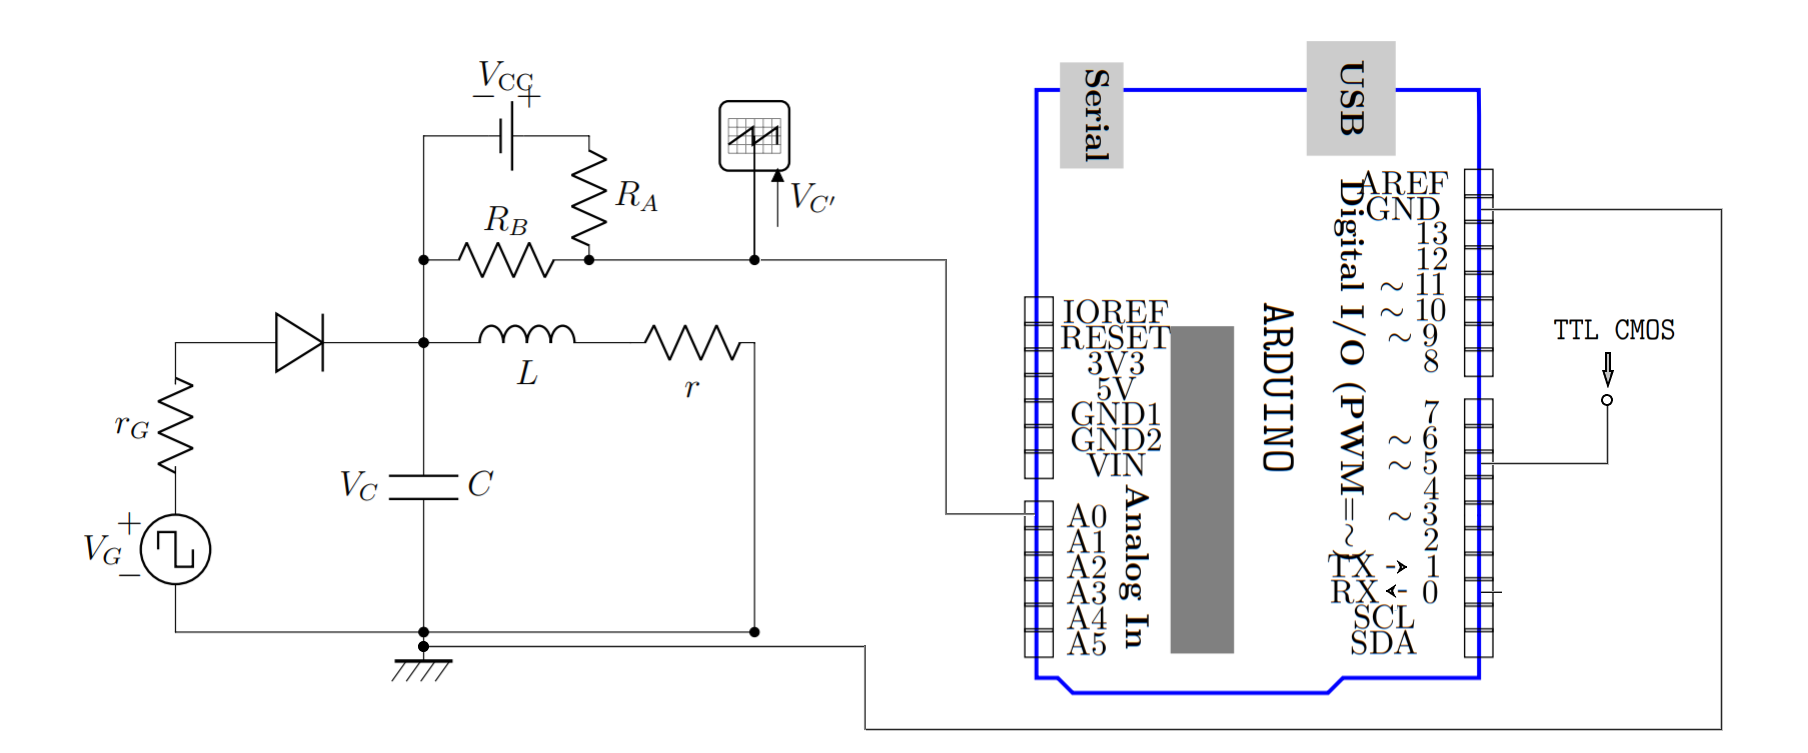
\includegraphics[width=14cm]{RLCschm}
	\caption{Diagramma del circuito RLC studiato\label{schm: RLC}}
\end{figure}

\subsubsection{Oscillatore a reazione con BJT}
Il potenziometro $R_p$ permette di variare la corrente di base $I_b$ 
del transistor, mentre per regolare la corrente di collettore $I_c$ si variano
le resistenze $R_c$ tra i valori nominali di $1 - 2.2 \pm 10 \% \; 
\si{\kilo\ohm}$. 

\begin{figure}[!htp]
	\centering 
		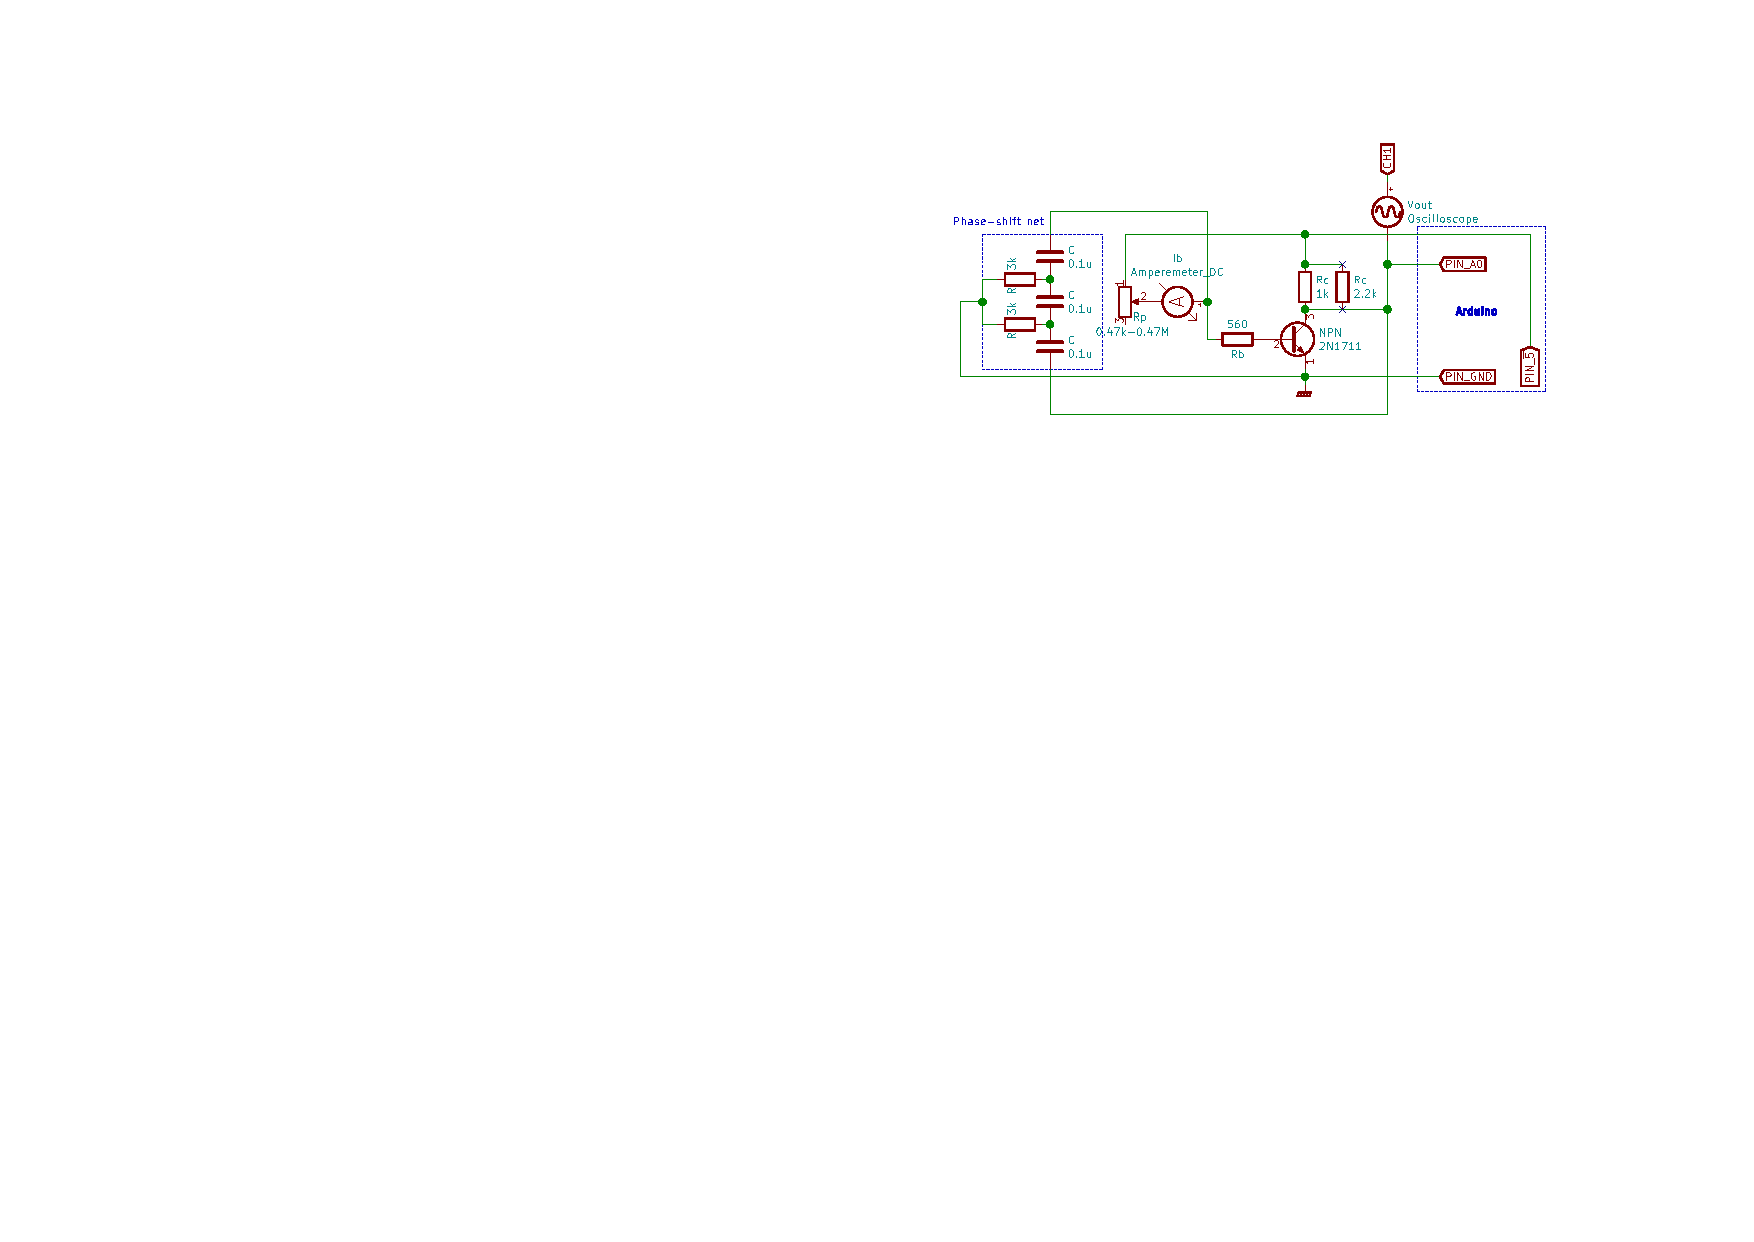
\includegraphics[width=14cm]{BJTschm}
	\caption{Schema circuitale dell'oscillatore a reazione con BJT
	studiato\label{schm: BJT}}
\end{figure}

%================================================================
%                   Analisi dati e Risultati
%================================================================
\section{Analisi dati e Risultati}
Inizialmente si sono convertite le acquisizioni e le incertezze associate in
d.d.p. tramite i fattori di conversione per l'ADC di \verb+Arduino+ per
$V_{\rm ref} = 5 \si{\V}$ standard TTL e $V_{\rm ref} = 1.1 \si{\V}$
interno, determinati con un semplice fit lineare.
\begin{align*}
	V_{\rm ref} &= 1.1\; \rm V	&V_{\rm ref} &= 5\; \rm V \\
	m_1 &= 1.040 \pm  0.006  \; \mathrm{mV/digit} 
	& m_5  &= 4.70 \pm 0.06  \; \mathrm{mV/digit} \\
	q_1 &= 1.5 \pm 1.6  \; \si{\mV} 	
	&q_5 &= 16  \pm 8  \; \si{\mV} \\
	\corr{m_1} {q_1} &= - 0.28      &\corr{m_5}{q_5} &= - 0.24 \\
	\chi^2/\text{ndof} &= 2.6/11	&\chi^2/\text{ndof} &= 0.7/11 \\ 
	\text{abs\_sigma} &= \rm True	&\text{abs\_sigma} &= \rm True
\end{align*}

\begin{figure}[!htb]
	\centering
	\begin{subfigure}{.5\textwidth}
		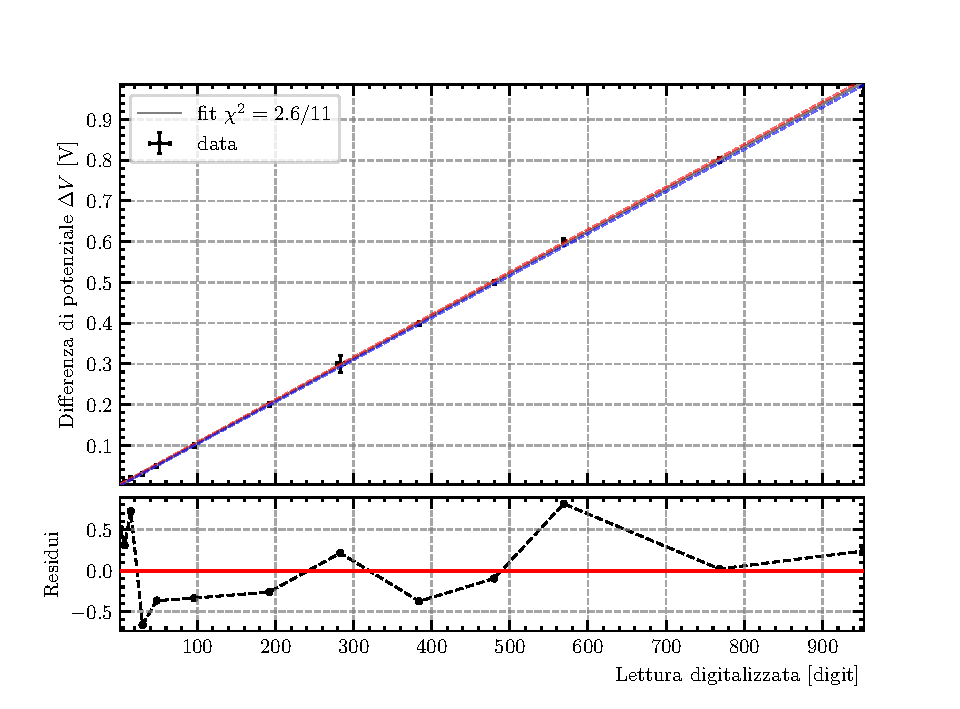
\includegraphics[width=8.5cm]{cal1.1}
		\caption{Calibrazione ADC per reference = \texttt{INTERNAL} $1.1 \si{\V}$. 
	\label{fig: cal1.1}}
	\end{subfigure}%
	\begin{subfigure}{.5\textwidth}
		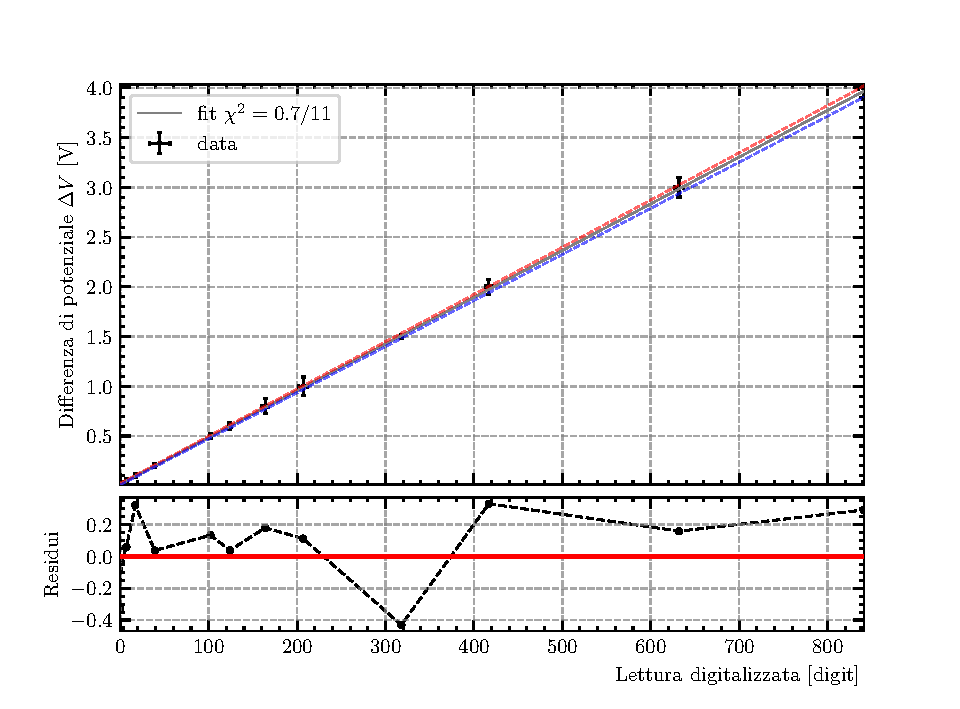
\includegraphics[width=8.5cm]{cal5}
		\caption{Calibrazione ADC per reference = \texttt{DEFAULT} $5 \si{\V}$. 
	\label{fig: cal5}}
	\end{subfigure}
	\caption{Risultato delle misure di calibrazione il pannello superiore mostra
		dati, retta ottenuta dal best-fit e "curve di confidenza", quello inferiore
		il grafico dei residui normalizzati.\label{fig: cals}}
\end{figure}

\subsection{Circuito RC}
Ricordando il guadagno atteso per un filtro RC passivo, dalla trasformata
di Fourier si riesce ad apprezzare l'effetto di attenuazione sulle armoniche
superiori dei segnali integrati per $f \gg f_T$.
\begin{figure}[!htb]
\centering
	\begin{subfigure}{.5\textwidth}
	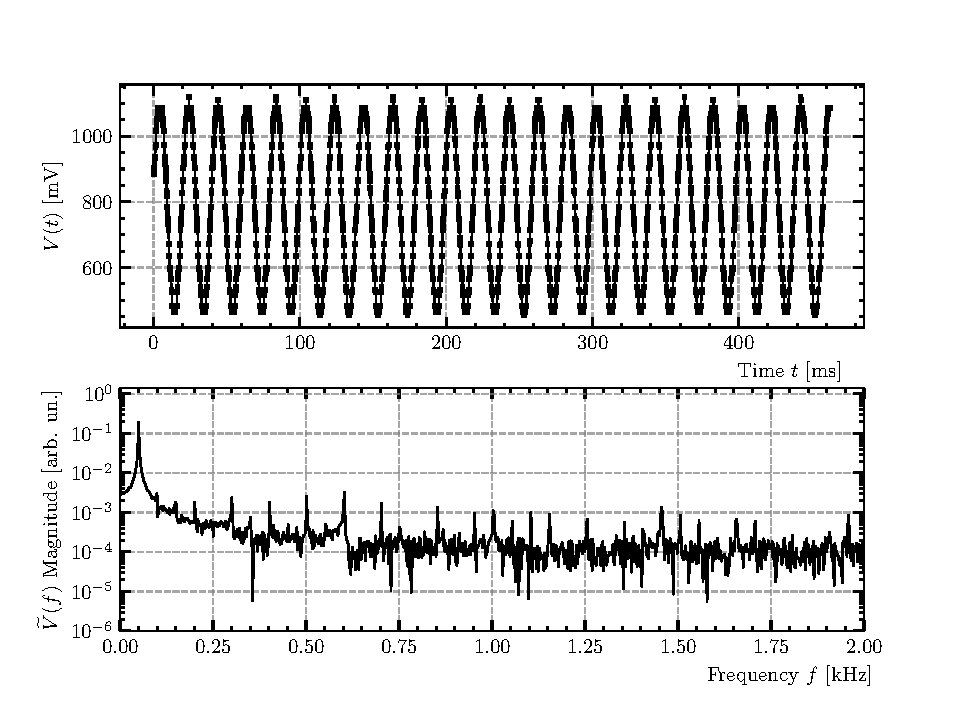
\includegraphics[width=8.5cm]{RCsin50}
	\caption{$\Delta t = 100 + 13 \pm 2 \si{\us} \; f = 50.01 \pm 0.01 \si{\Hz}$}
	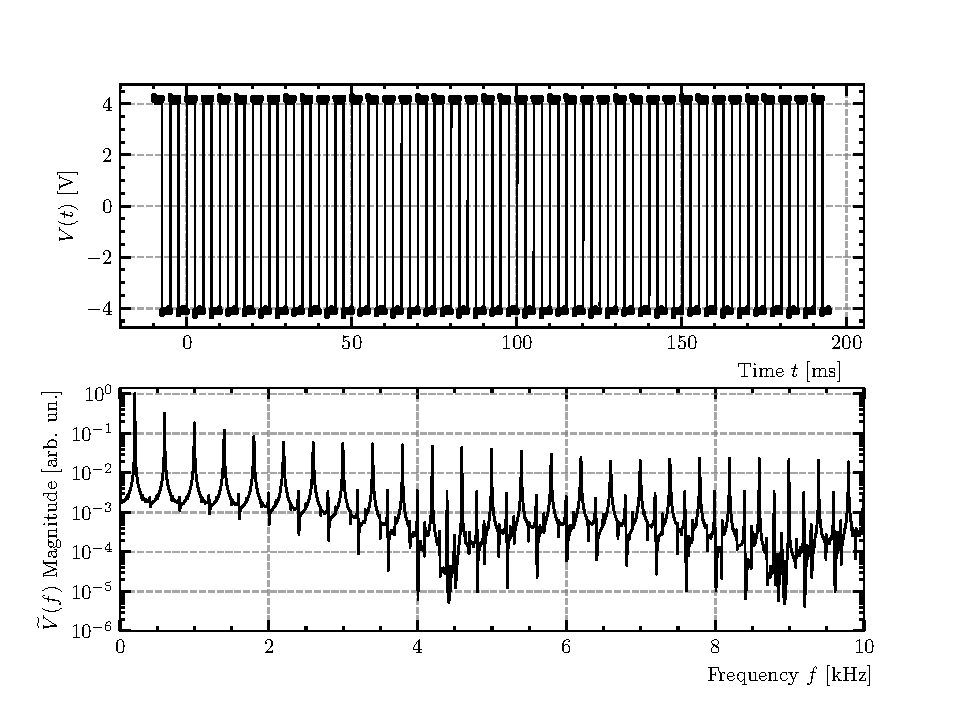
\includegraphics[width=8.5cm]{DSOsqw200}
	\caption{$\Delta t = 2 \pm 100 \si{ppm \, \us}$ (nom.)
	$\; f = 199.80 \pm 0.01 \si{\Hz}$}
	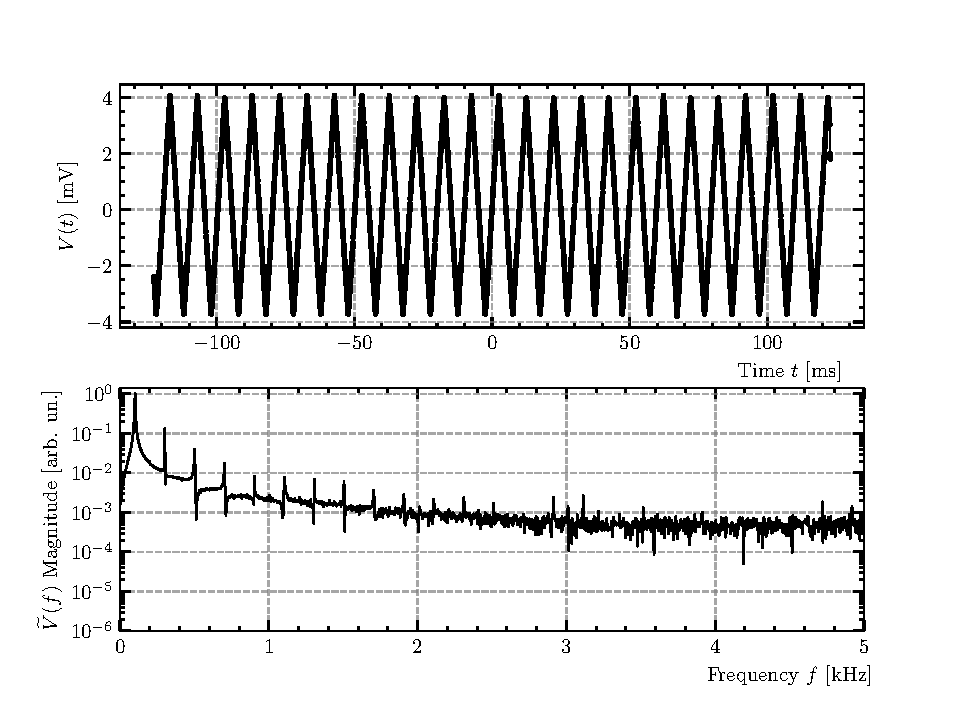
\includegraphics[width=8.5cm]{RCtrg100}
	\caption{$\Delta t = 20 \pm 100 \si{ppm \, \us}$ (nom.)
	$ \; f = 100.50 \pm 0.02 \si{\Hz}$}
\label{fig: RCin}
	\end{subfigure}%
	\begin{subfigure}{.5\textwidth}
	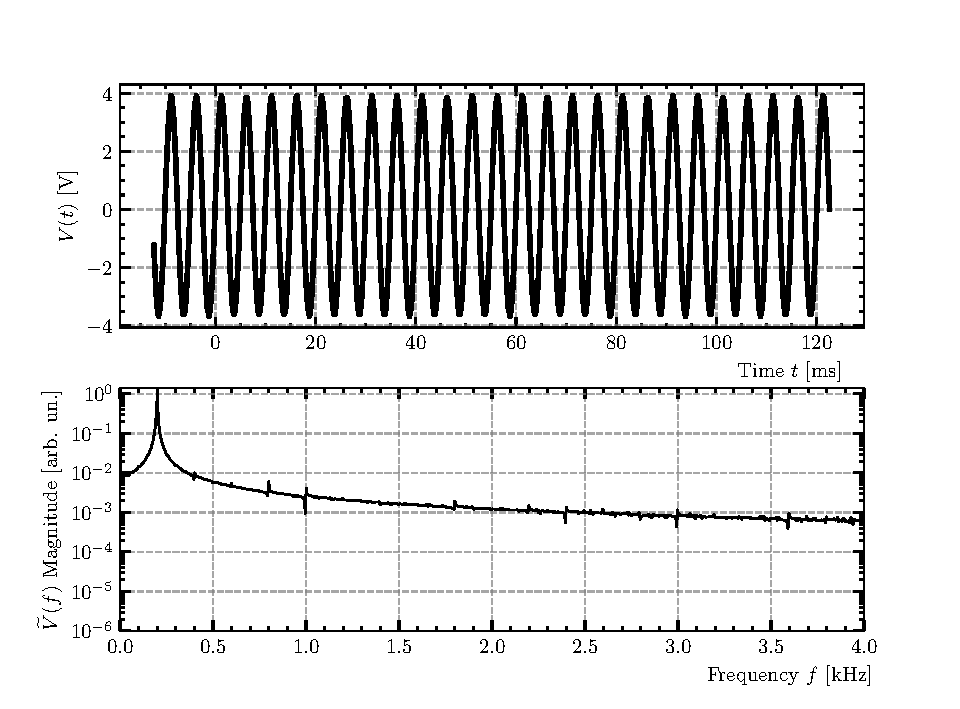
\includegraphics[width=8.5cm]{DSOsin200}
	\caption{$\Delta t = 2 \pm 100 \si{ppm \, \us}$ (nom.)
	$\; f = 199.68 \pm 0.01 \si{\Hz}$}
	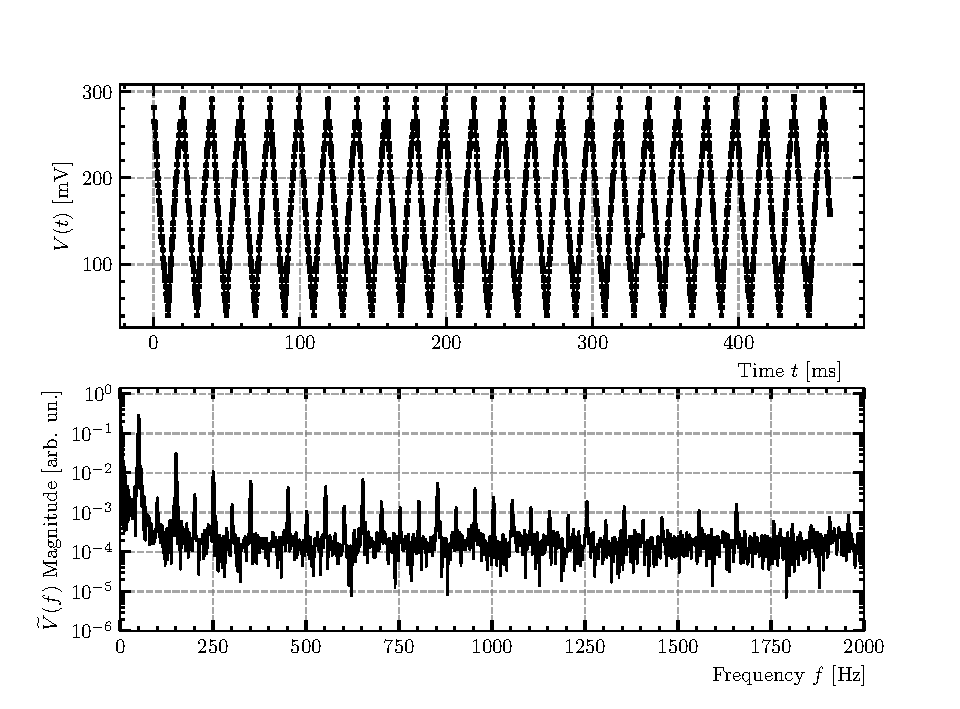
\includegraphics[width=8.5cm]{RCfin50}
	\caption{$\Delta t = 100 + 13 \pm 2 \si{\us} \; f = 50.51 \pm 0.02 \si{\Hz}$}
	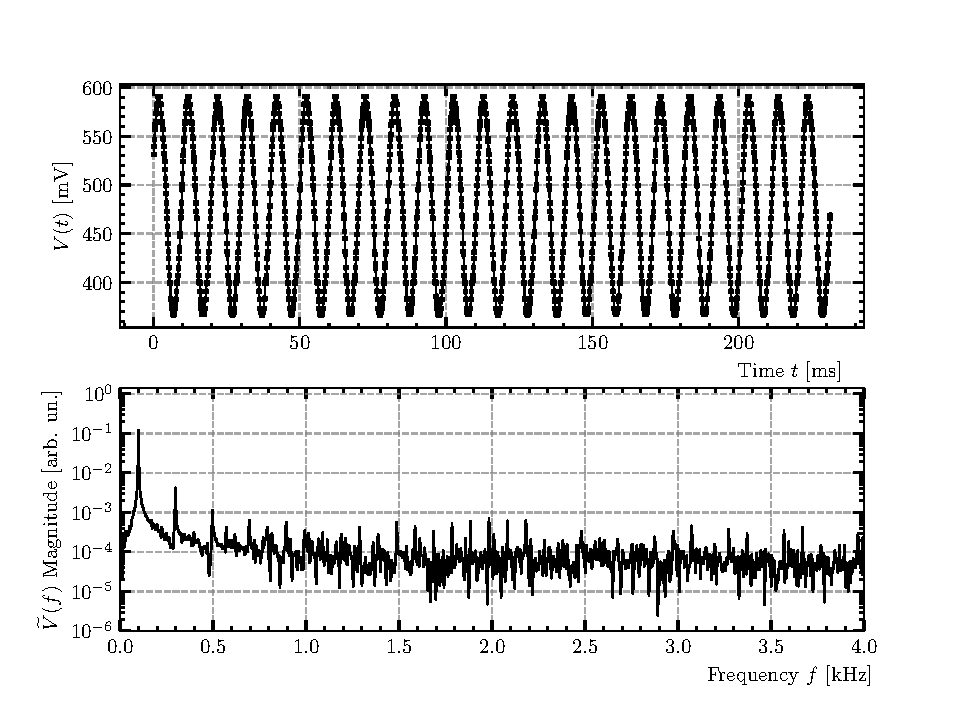
\includegraphics[width=8.5cm]{RCpar100}
	\caption{$\Delta t = 100 + 13 \pm 2 \si{\us} \; f = 99.10 \pm 0.04 \si{\Hz}$}
\label{fig: Rcint}
	\end{subfigure}%
	\caption{Risultati trovati sull'effetto dell'integratore RC sui segnali
			nel tempo e sulla loro trasformata di Fourier. A sinistra le
			onde in ingresso seno, quadra e triangolare e a destra i corrispondenti 
		 	segnali filtrati. \label{fig: RCall}}
\end{figure}

\subsection{Circuiti RLC}
\begin{figure}[!htb]
\centering
	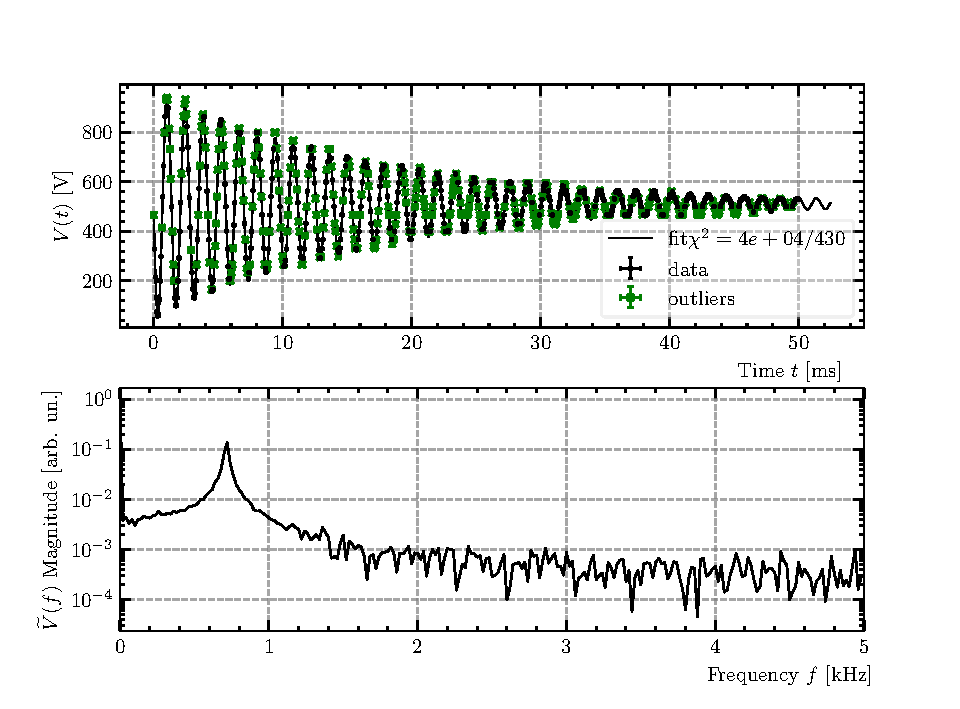
\includegraphics{RLC0.1b4}
	\caption{Illustrazione del picco che si trova nei dati campionati
			in fondo all'oscillazione smorzata del circuito, ovviamente
			non prevista dal modello di best fit. 
			$\Delta t = 50 + 13 \pm 3 \; [\si{\us}]$ $f = 715.15 \pm 2 \si{\Hz}$
			$C = 0.1 \pm 10\% \; [\si{\micro\F}]$ $L = 0.5 \pm 10 \% \;
			[\si{\henry}]$ $r = 58 \pm 10\%	\; [\si{\ohm}]$.
			$Q_f = 62$.	\label{fig: RLC0.1b5}}
\end{figure}

Alla fine del segnale oscillante\footnote{alla fine del
semiperiodo negativo dell'onda quadra in uscita dal generatore di funzioni}
si riesce ad apprezzare un picco positivo di circa $100$ digit $\approx 104$ mV,
questo coincide esattamente con il fronte di salita dell'onda quadra in
ingresso al circuito RLC.
Quando l'onda passa da LOW a HIGH, la corrente che scorre negli avvolgimenti
dell'induttore passa da un intensità trascurabile a $100 \si{\micro\A}$.
Dunque, secondo la legge degli induttori la bobina genera una tensione
proporzionale alla variazione dell'intensità di corrente:
$\Delta V(t) = L \frac{\ud I}{\ud t}$
il picco finale allora si deve alla stessa tensione che dà inizio
all'oscillazione, però di segno opposto; però ora il circuito non inizia
ad oscillare perché il diodo è in conduzione.
Un secondo possibile contributo al picco di tensione alla
fine del segnale oscillante è dato dalla capacità parassita
della giunzione PN, che possiamo  modellare come un condensatore
in parallelo al diodo. Quando il fronte d'onda sale rapidamente, parte
dell'onda quadra viene "lasciata passare" dal condensatore, ma da 
una simulazione con LTSpice ed una capacità (zero bias) nominale per
il diodo a giunzione \texttt{1N194}: $Cjo = 4 \si{\pico\farad}$
il contributo al picco finale risulta dell'ordine di qualche $\si{\nano\V}$.
Dunque l'effetto dell'accoppiamento capacitivo risulta decisamente trascurabile
rispetto alla risoluzione del sistema di acquisizione.
\begin{figure}[!htb]
\centering
	\begin{subfigure}{.5\textwidth}
		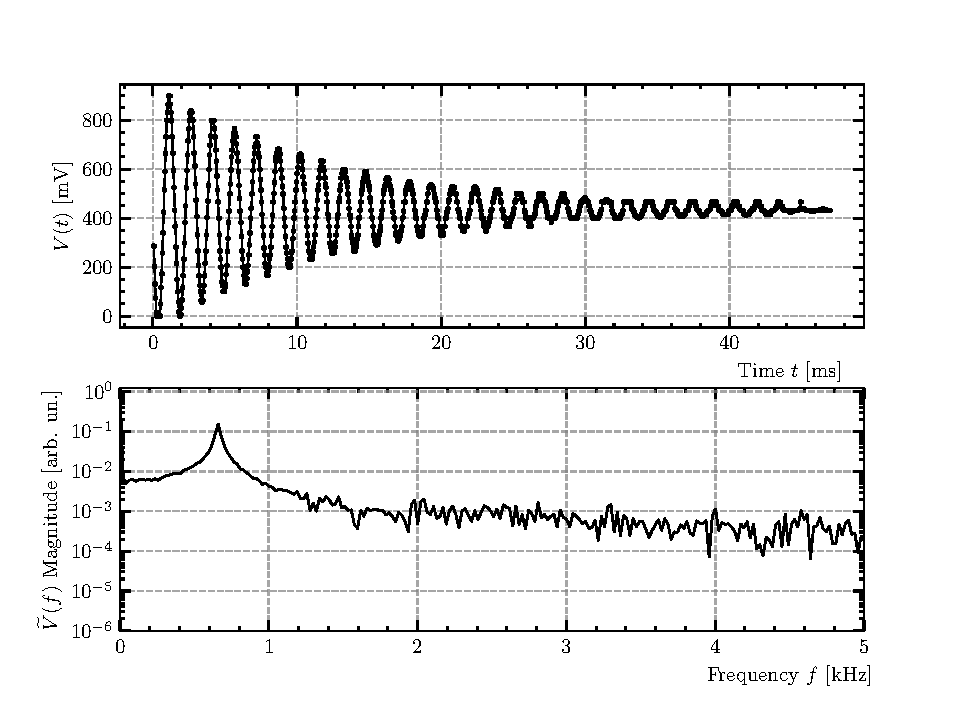
\includegraphics[width=8.5cm]{RLC0.1b3_net} 
	\caption{$\Delta t = 30 + 13 \pm 2 \si{\us} \; C = 0.1
			\pm 10 \% \si{\micro\F}$}
		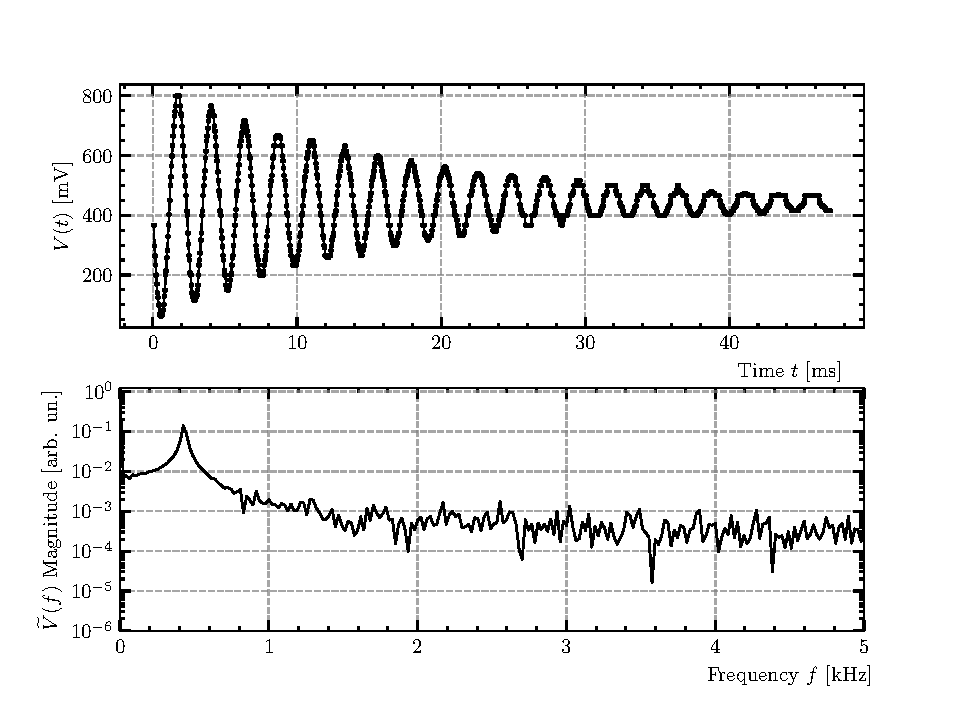
\includegraphics[width=8.5cm]{RLC0.22b3} 
	\caption{$\Delta t = 30 + 12 \pm 3 \si{\us} \; C = 0.22 
			\pm 10 \% \si{\micro\F}$}
		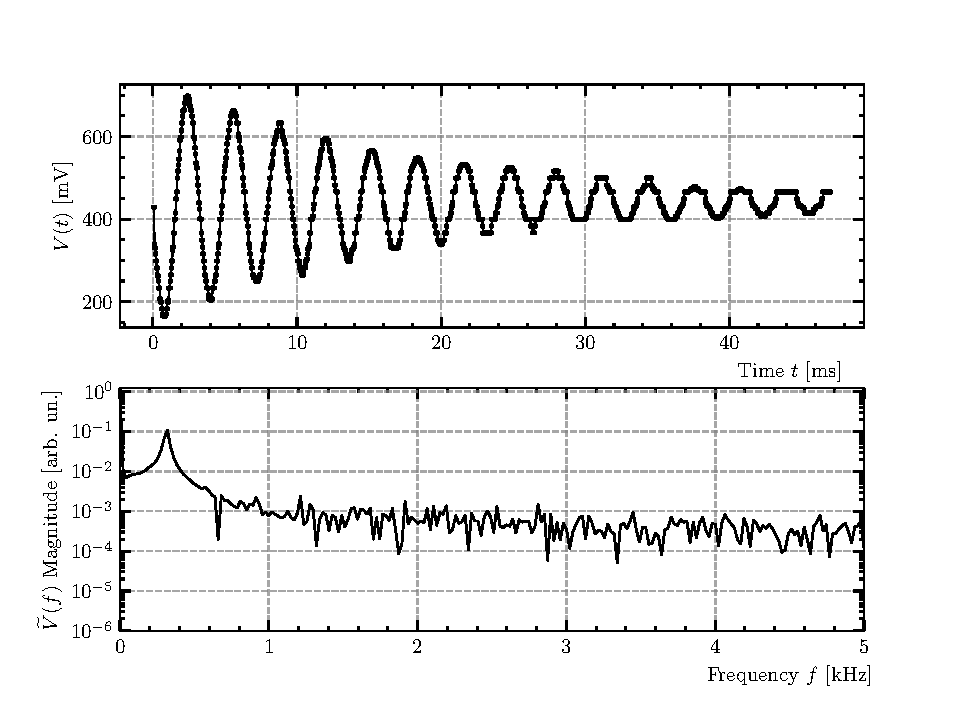
\includegraphics[width=8.5cm]{RLC0.47b3} 
	\caption{$\Delta t = 30 + 12 \pm 3 \si{\us} \; C = 0.47
			\pm 10 \% \si{\micro\F}$}
	\end{subfigure}%
	\begin{subfigure}{.5\textwidth}
		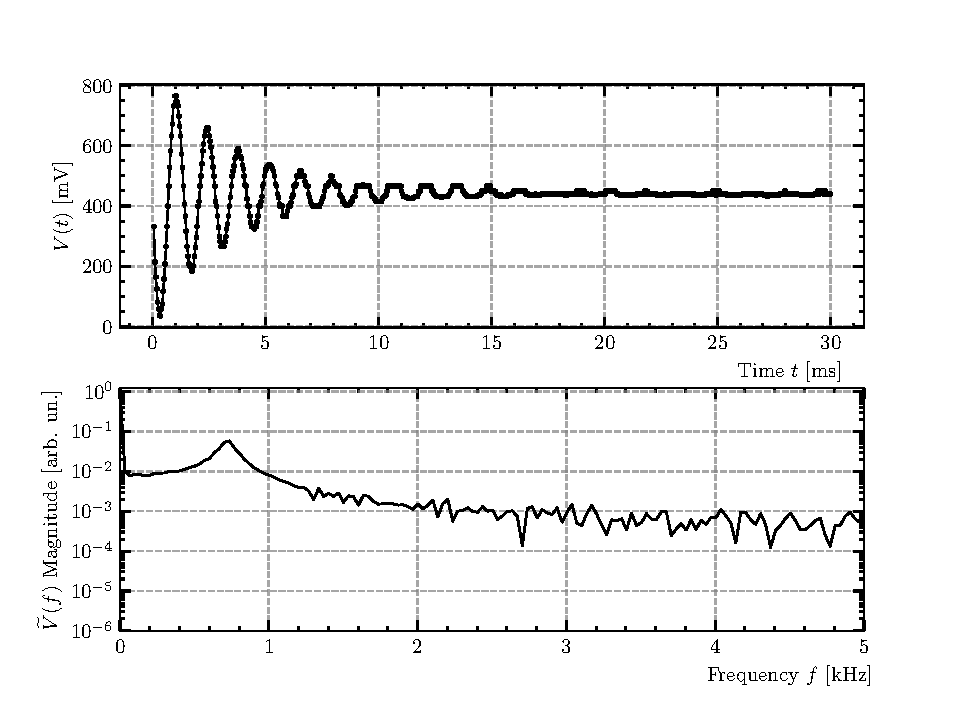
\includegraphics[width=8.5cm]{RLC0.1b3_traf}
	\caption{$\Delta t = 30 + 12 \pm 3 \si{\us} \; C = 0.1
			\pm 10 \% \si{\micro\F}$}
		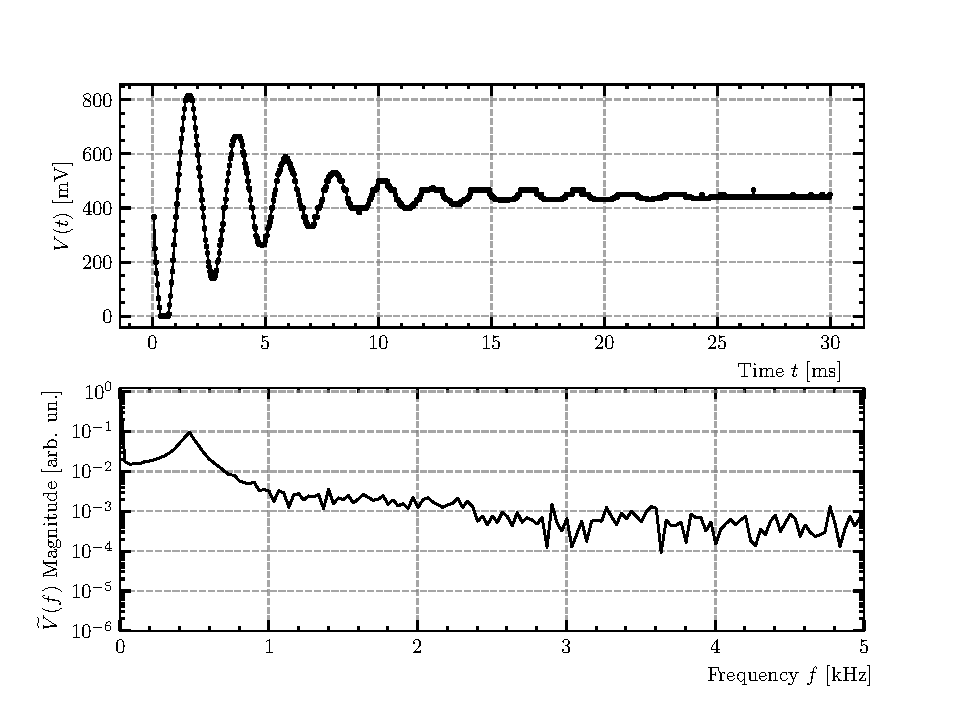
\includegraphics[width=8.5cm]{RLC0.22b3_traf}
	\caption{$\Delta t = 30 + 12 \pm 3 \si{\us} \; C = 0.22
			\pm 10\% \si{\micro\F}$}
		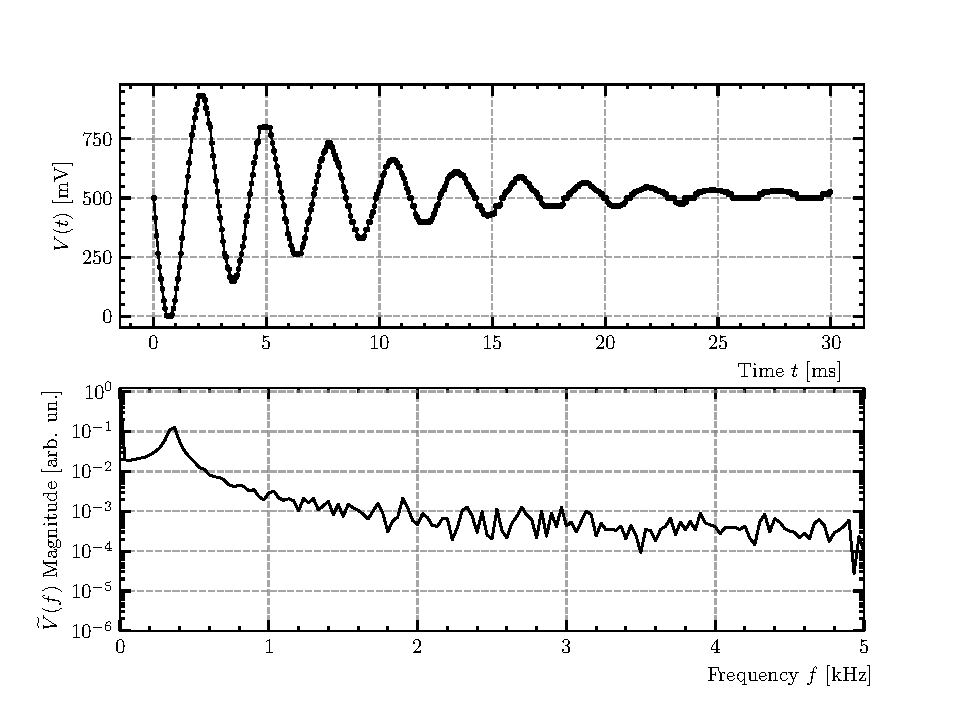
\includegraphics[width=8.5cm]{RLC0.47b5_all}
	\caption{$\Delta t = 50 + 13 \pm 3 \si{\us} \; C = 0.47
			\pm 10 \% \si{\micro\F}$}
	\end{subfigure}%
	\caption{Risultati sugli effetti dovuti ai diversi nuclei inseriti
			all'interno dell'induttore sulla larghezza di riga della trasformata
			e sul segnale in uscita dall'oscillatore RLC. Nella colonna sinistra
			lasciato vuoto, a destra con un blocco pieno di alluminio.
			 \label{fig: RLCall}}
\end{figure}

\begin{table}[!htb]
\begin{center}
\begin{tabular}{cc||cccc}
	\toprule
	Nucleo & $C\; \pm 10 \% [\si{\micro\F}]$ & $f_0 [\si{\Hz}]$ & $\tau [\si{\ms}]$ 
	& $L \pm 10 \% [\si{\henry}]$ & $Q_f$ \\
	\midrule
	\midrule
	 & $0.1$ & $659.73 \pm 0.02$ & $12.52 \pm 0.02$ & $0.53$ & $28$ \\
	Aria & $0.22$ &$431.69 \pm 0.03$ & $ 16.55 \pm 0.03$ & $0.52$ & $23$ \\
	 & $0.47$ & $325.41 \pm 0.01$ & $21.98 \pm 0.03$ & $0.51$ & $18$ \\ 
	\midrule
	 & $0.1$ & $790.25 \pm 0.07$ & $5.19 \pm 0.01$ & $0.41$ & $13$\\
	Alluminio & $0.22$ & $517.60 \pm 0.09$ & $6.54 \pm 0.02$ & $0.43$ & $10 $ \\
	 & $0.47$ & $353.51 \pm 0.06$ & $7.88 \pm 0.02$ & $0.44$ & $8$ \\
	\bottomrule
\end{tabular}
\caption{Risultati trovati, dall'analisi di spettro e nel dominio del tempo,
degli effetti sulla qualità dell'oscillazione dovuti a nuclei di materiale
diverso nel cuore dell'induttore. \label{tab: RLC}}
\end{center}
\end{table}

L'oscillazione RLC è modulata da una forzante a forma di onda quadra a
$f = 10 \si{\Hz}$ che equivale all'azione di un sistema di chopping
meccanico\footnote{Ovviamente senza le complicazioni legate alle
fluttuazioni introdotte dal movimento \emph{jitter} meccanico.}
tipicamente usato negli esperimenti di fluorescenza. Se la frequenza del
segnale oscillante avesse una frequenza troppo bassa (a causa del rumore
$1/f$) per filtrare il rumore da cui è affetta la misura, potremmo usare
il Lock-in-Detector sincronizzando i segnali di riferimento con l'onda quadra,
per migliorare il Signal to Noise Ratio (SNR).

\subsection{Oscillatore a reazione con BJT}
La dipendenza non lineare tra tensione e corrente della curva caratteristica
di base del transistor porta ad una distorsione asimmetrica del segnale, 
qualitativamente diversa da un'onda sinusoidale nel dominio del tempo.
Infatti il contenuto armonico della trasformata di $V_{\text{out}}$ risulta
caratterizzato da un intervallo di frequenze a cui il circuito può
oscillare. Un contributo alle armoniche superiori osservate nella FFT
potrebbe essere dato dalla bassa qualità della rete di sfasamento,
in effetti la larghezza a metà altezza intorno alla frequenza
fondamentale risulta $\Delta \omega_{\text{FWHM}} = 0.4 - 0.5$. 
\begin{figure}[!htb]
\centering
	\begin{subfigure}{.5\textwidth}
	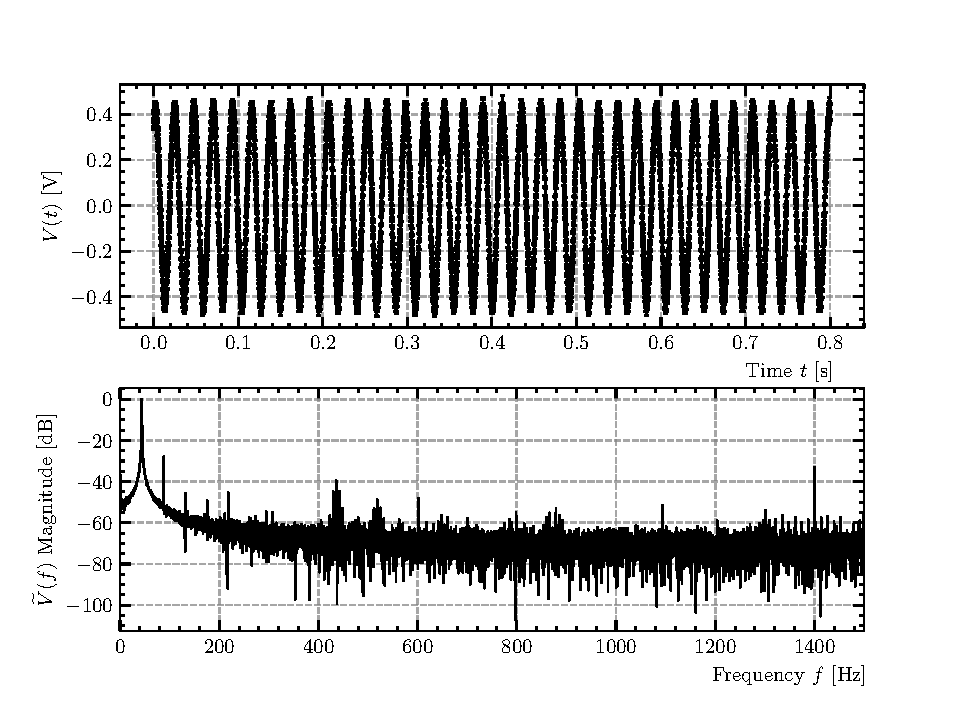
\includegraphics[width=8.5cm]{DSObjt44}
	\caption{$\Delta t = 200 \pm 0.01 \% \si{\us} \; f = 43.87
	\pm 0.04 \si{\Hz} \; I_b = 0.98 \pm 0.04 \si{\uA}$}
	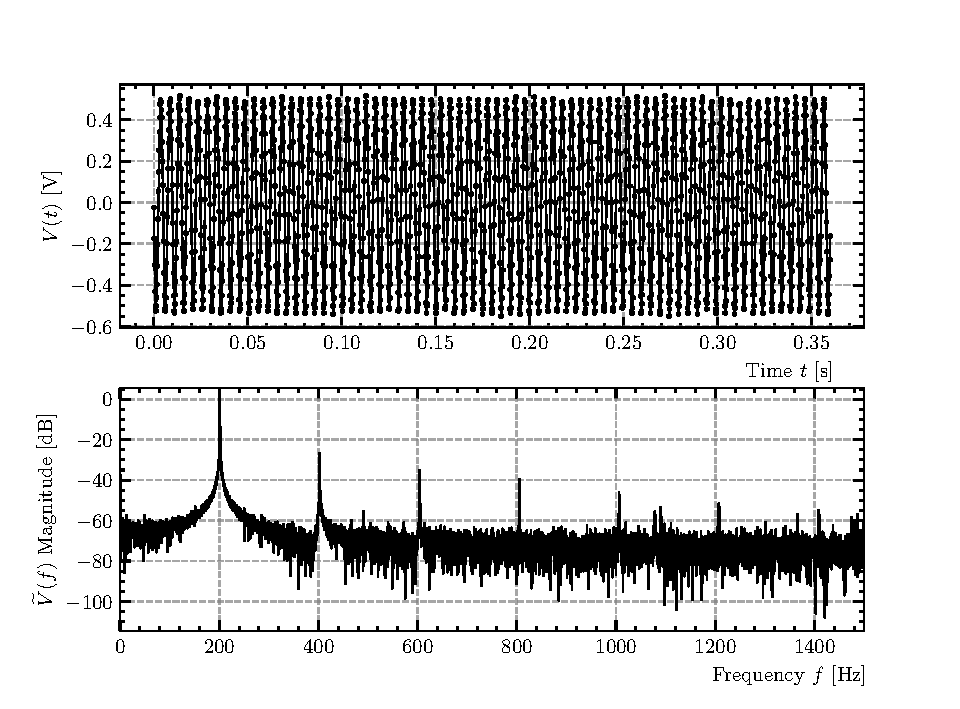
\includegraphics[width=8.5cm]{DSObjt201}
	\caption{$\Delta t = 100 \pm 0.01 \% \si{\us} \; f = 201.22
	\pm 0.02 \si{\Hz} \; I_b = 1.20 \pm 0.06 \si{\uA}$}
	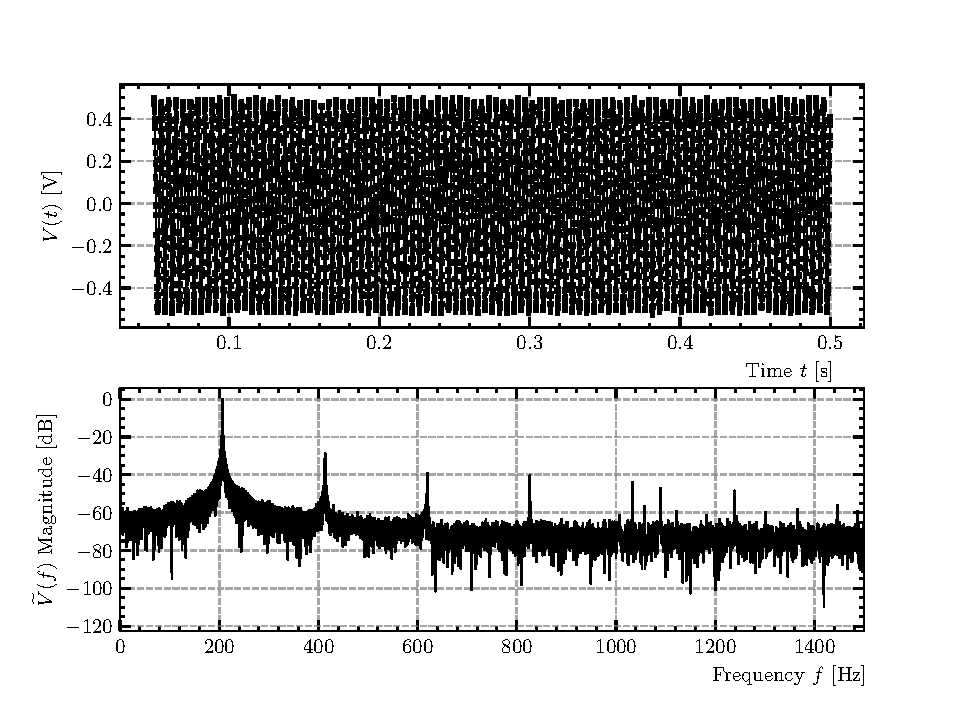
\includegraphics[width=8.5cm]{DSObjt206}
	\caption{$\Delta t = 200 \pm 0.01 \% \si{\us} \; f = 206.65
	\pm 0.01 \si{\Hz} \; I_b = 1.27 \pm 0.06 \si{\uA}$}
\label{fig: BJTin}
	\end{subfigure}%
	\begin{subfigure}{.5\textwidth}
	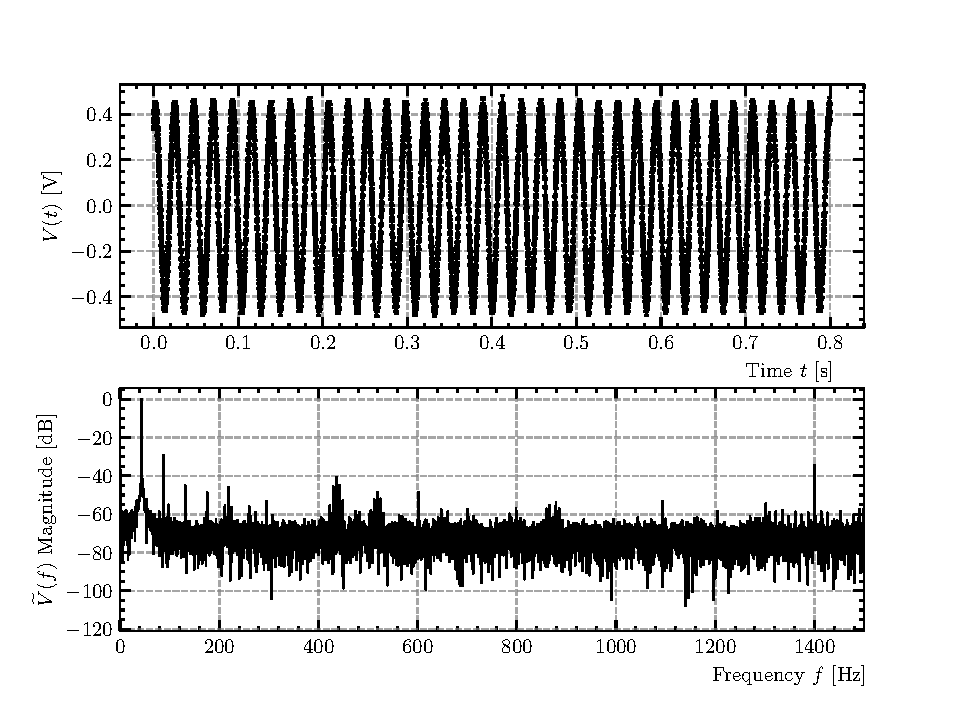
\includegraphics[width=8.5cm]{DSObjt44hamm}
	\caption{Finestra di Hamming ($a_0 = 0.54, \, a_1 = 0.46$).}
	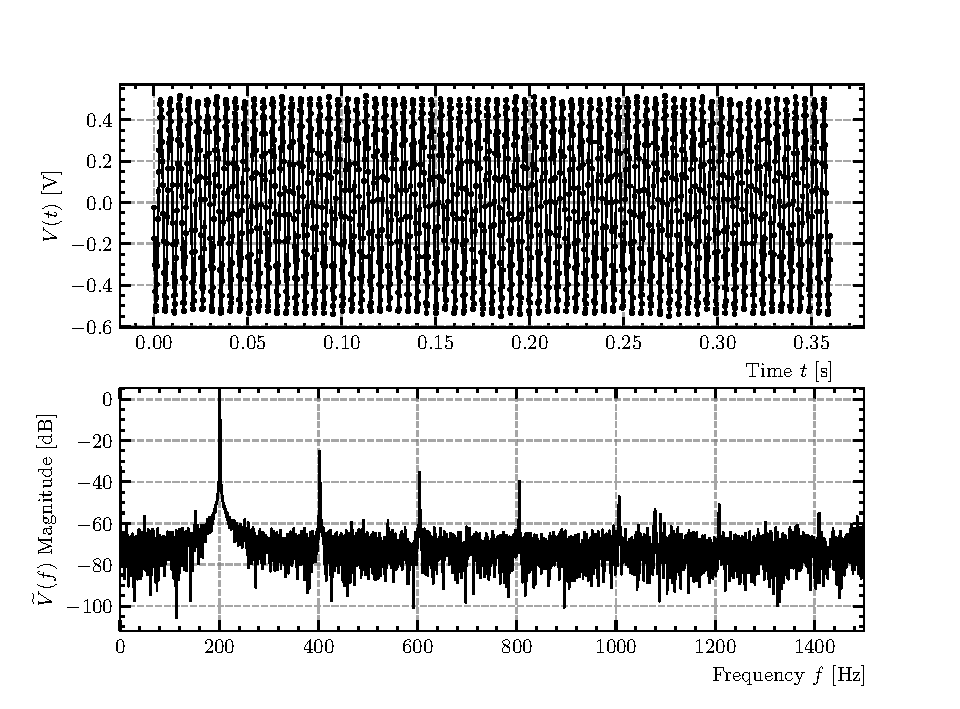
\includegraphics[width=8.5cm]{DSObjt201blak}
	\caption{Finestra di Blackman ($a_0 = 0.42, \, a_1 = 0.5, \, a_2 = 0.08$).}
	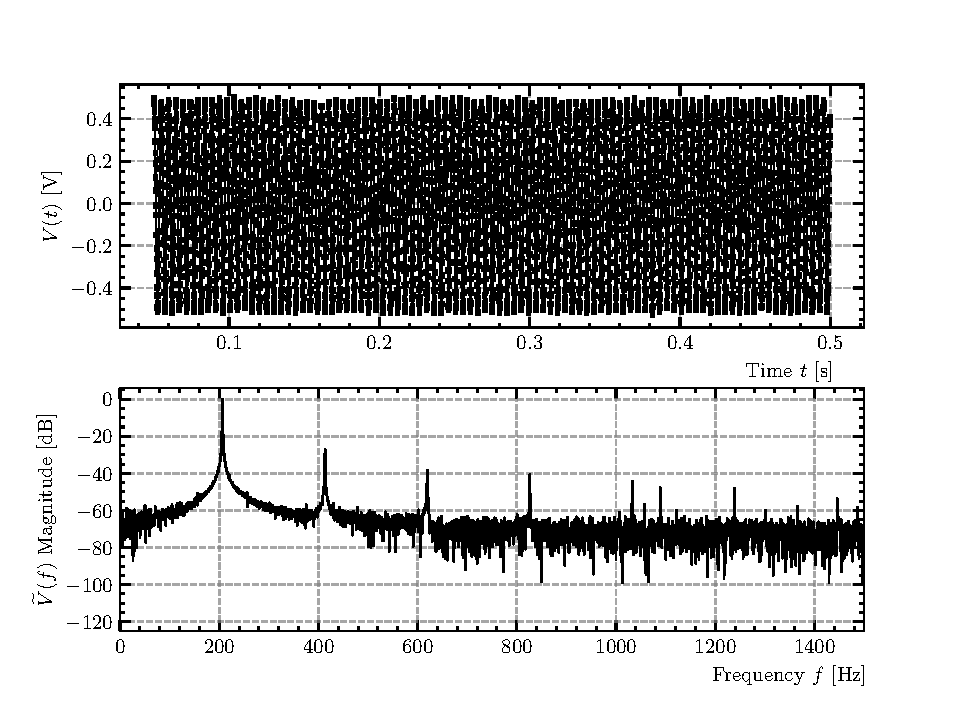
\includegraphics[width=8.5cm]{DSObjt206bart}
	\caption{Finestra di Bartlett o triangolare.}
\label{fig: BJTwin}
	\end{subfigure}%
	\caption{Risultati trovati sull'effetto di diverse finestre	sulle
			perdite di spettro nella trasformata del segnale in uscita
		 	dall'oscillatore a reazione.
			Nella colonna sinistra prima, a destra dopo aver applicato
			le funzioni finestra al segnale. \label{fig: BJTall}}
\end{figure}

\subsection{Detezione sincrona}
Intendiamo estrarre un segnale $V(t)$ relativamente piccolo
in presenza di rumori -forti- e di natura diversa:
Un rumore di pick-up magnetico a $f_{\text{pu}} = 50 \si{\Hz}$ e ampiezza
$A_{\text{pu}} = 2$ [arb. un.], una tensione costante pari a 
$V_{\text{CC}} = 2.5$ [arb. un.] ed un rumore -bianco-, che possiamo modellare
con un generatore di numeri pseudo-casuali distribuiti normalmente
intorno a 0 con deviazione standard $\sigma = 10$ [arb. un.].
In queste condizioni non è possibile distinguere il piccolo segnale $V(t)$ 
di ampiezza $V_{\text{sig}} = 0.1$, [arb. un.], frequenza 
$f = 1 \si{\kilo\hertz}$ e fase costante $\phi = 0.2 \; \si{rad}$
dal rumore neanche analizzando lo spettro in frequenza:
\begin{figure}[!htb]
\centering
	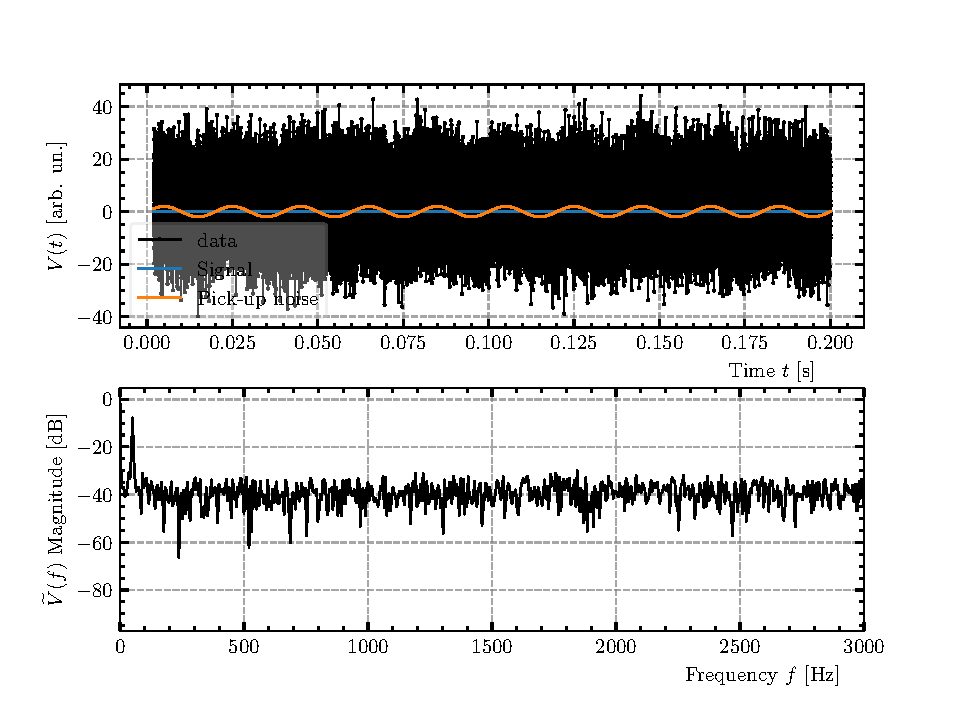
\includegraphics{LIA1k}
	\caption{Nel pannello superiore il segnale rumoroso e sotto la sua
			trasformata di Fourier, in cui si notano la componente a
			$50 \si{\Hz}$ del pick-up e la componente DC, ma non il segnale
			d'interesse a $1 \si{\kilo\hertz}$. \label{fig: LIAnoise}}
\end{figure}
Usando la tecnica di detezione omodina è possibile ricostruire fase,
ampiezza e frequenza di $V(t)$, isolandolo dal rumore asincrono e fuori
fase rispetto ai riferimenti ed al segnale stesso:
\begin{figure}[!htb]
	\centering
	\begin{subfigure}{.5\textwidth}
		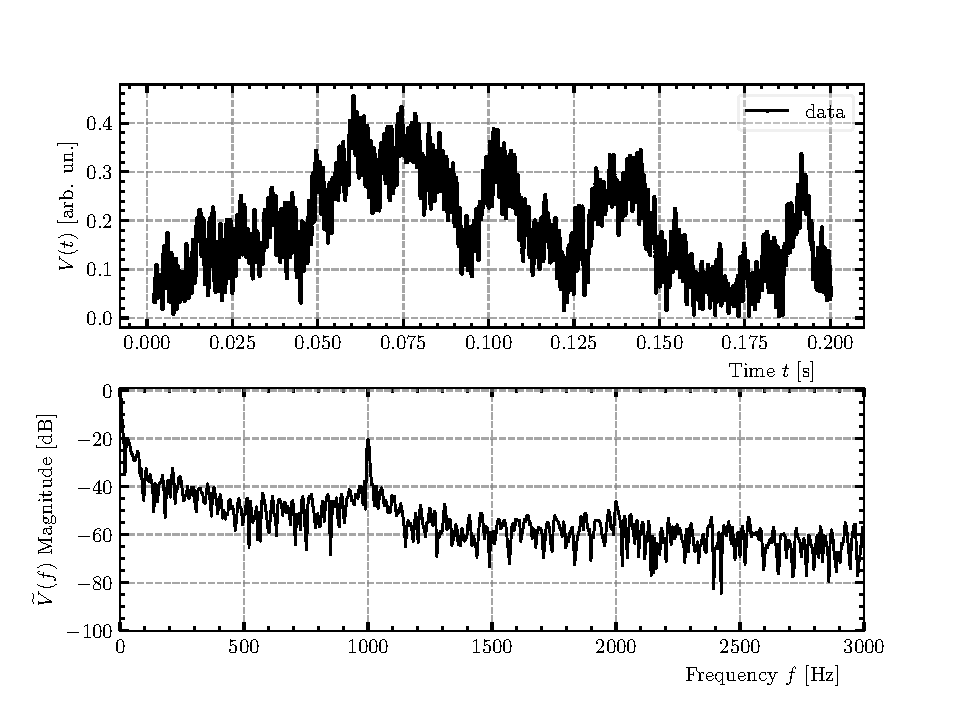
\includegraphics[width=8.5cm]{LIAFFT1k}
		\caption{Nel pannello superiore l'ampiezza di $V(t)$ in uscita dal LIA \\
				\; e sotto la sua trasformata di Fourier.}
	\end{subfigure}%
	\begin{subfigure}{.5\textwidth}
		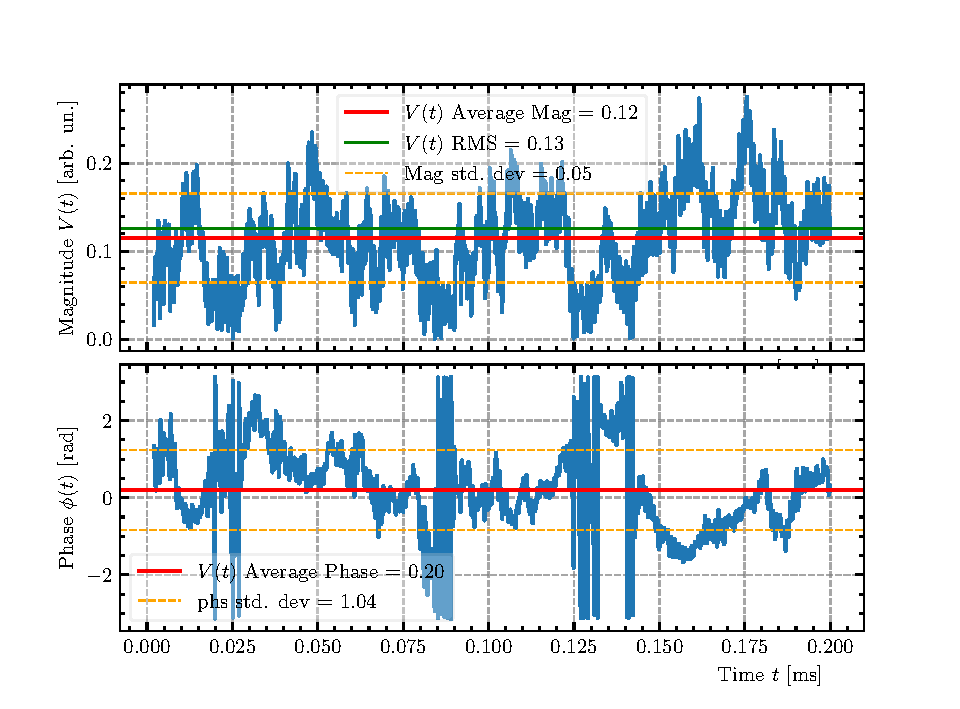
\includegraphics[width=8.5cm]{LIAmag1k}
		\caption{Ampiezza e fase di $V(t)$ trovate dal Lock-In-Detector.}
	\end{subfigure}
	\caption{Risultato della simulazione di detezione sincrona di un segnale
			affetto da rumori di ampiezze superiori di alcuni ordini di
			grandezza SNR $\approx 10^{-2}$. Per la misura si è scelto un
			intervallo di campionamento abbastanza breve per ridurre
			gli effetti dovuti alla rappresentazione discreta del segnale
			nel tempo, $\Delta t = 2 \si{\us}$ ed un tempo totale di
			"acquisizione" $T_{\text{mis}} = 200 \si{\ms}$.
		\label{fig: LIAall}}
\end{figure}
Adesso una misura del segnale è possibile e, quanto il rivelatore simulato è
riuscito a dedurre sul nostro segnale non dista più del $20 \%$ rispetto ai
valori attesi impostati nello script $V_{\text{mis}} \approx 0.12 \;
\si{arb. un.} \leadsto V_{\text{sig}}$ $\phi_{\text{mis}} \approx 0.2 \;
\si{rad} \leadsto \phi$.

\subsection{Nota sull'implementazione}
Per determinare i parametri ottimali e le rispettive covarianze si \`e
implementato in \verb+Python+ un algoritmo di fit basato sui minimi quadrati
mediante la funzione \emph{curve\_fit} della libreria 
\texttt{SciPy}\cite{scipy}.
Per tutti i fit su campionamenti digitali di \verb+Arduino+ si \`e imposto
$\rm{abs\_sigma} =$ True, avendo preso come incertezza associata il valore
convenzionale $\sigma = 1$ digit, per cui effettivamente si sta eseguendo
un fit dei minimi quadrati. Per tutti gli altri campionamenti, in cui la
sorgente principale di incertezza abbia natura non statistica o non meglio
determinata si è posto $\rm{abs\_sigma} =$ False. 
Il modulo \texttt{signal} della stessa libreria è stato usato per
la realizzazione dei filtri numerici e delle finestre, mentre
l'implementazione dell'algoritmo per il calcolo della FFT è lo stesso
definito dalla libreria \texttt{NumPy}\cite{numpy}.
Si rimanda ai
\href{https://github.com/BernardoTomelleri/FFT/tree/master}{sorgenti}
per ulteriori informazioni sugli script utilizzati, dove \verb+lab.py+ funge
da libreria di funzioni di appoggio e \verb+data.py+ definisce i parametri
fondamentali in ingresso per l'analisi dei dati.
\subsubsection{Filtro outliers}
Per rimozione degli outlier si intende lo scartare tutti quei punti che
distano dal valore atteso per la misura $y$: $E[y] := \mu_y$ pi\`u di una
soglia arbitraria $k$ di incertezze associate $\Delta y$
(nel nostro caso \`e stato scelto $k = 5$).

%================================================================
%                          Conclusioni
%================================================================
\section{Conclusioni}
Sì è visto l'andamento decrescente delle componenti armoniche di un segnale
all'aumentare della frequenza causato da un filtro passa-basso.
Si è osservata una correlazione fra larghezza di riga della curva di risonanza
e lo smorzamento presente in un circuito oscillante RLC.
Si è riusciti ad apprezzare l'effetto della risposta non lineare
dell'amplificatore invertente (BJT a emettitore comune) sullo spettro
in frequenza dell'auto-oscillazione e l'uso di diverse finestre per
rimdediare gli effetti di perdita spettrale.
Si è illustrato uno dei vantaggi del metodo di Lock-in-Detection per 
la risoluzione di segnali sommersi da rumore di ampiezze maggiori di alcuni
ordini di grandezza.

%================================================================
%                            END
%================================================================
\medskip
\bibliographystyle{IEEEtrandoi}
\bibliography{refs}
\end{document}
